\documentclass[journal]{IEEEtran}
\usepackage{fix-cm}

\usepackage{array}
\usepackage[caption=false,font=normalsize,labelfont=sf,textfont=sf]{subfig}
\usepackage{textcomp}
\usepackage{stfloats}
\usepackage{url}
\usepackage{verbatim}
\usepackage{graphicx}
\usepackage{xcolor}
\usepackage{amsmath}
\usepackage{amssymb}
\usepackage{amsthm}
\usepackage{booktabs}
\usepackage{multirow}
\usepackage{cite}
\usepackage{orcidlink}
\usepackage{msc}
\usepackage{tikz}
\usetikzlibrary{arrows.meta,calc,positioning,shapes.symbols,backgrounds,decorations.pathmorphing}
\usepackage{pgfplots}
\pgfplotsset{compat=1.18}
\hyphenation{op-tical net-works semi-conduc-tor IEEE-Xplore}

% ---------------- theorem environments ----------------
\theoremstyle{plain}
\newtheorem{theorem}{Theorem}
\newtheorem{lemma}{Lemma}
\theoremstyle{definition}
\newtheorem{definition}{Definition}

% ---------------- notation (sans-serif identifiers) ----------------
\newcommand{\Veh}{\mathsf{V}}            % vehicle
\newcommand{\Fog}{\mathsf{F}}            % fog node
\newcommand{\CS}{\mathsf{CS}}            % cloud server
\newcommand{\Adv}{\mathcal{A}}           % adversary
\newcommand{\SK}{\mathsf{SK}}            % session key
\newcommand{\VID}{\mathsf{VID}}          % vehicle identity
\newcommand{\FID}{\mathsf{FID}}          % fog identity
\newcommand{\CID}{\mathsf{CID}}          % cloud identity
\newcommand{\VPW}{\mathsf{VPW}}          % password
\newcommand{\HPW}{\mathsf{HPW}}          % masked password
\newcommand{\TV}{\mathsf{TV}}            % verifier
\newcommand{\Cred}{\mathsf{Cred}}        % protected credentials
\newcommand{\RL}{\mathsf{RL}}            % revocation list
\newcommand{\PV}{\mathsf{PV}}            % notation of [12]
\newcommand{\MV}{\mathsf{MV}}
\newcommand{\RID}{\mathsf{RID}}
\newcommand{\PFD}{\mathsf{PFD}}
\newcommand{\Rb}{\mathsf{Rb}}
\newcommand{\RK}{\mathsf{RK}}
\newcommand{\h}{\mathsf{h}}              % hash function
\newcommand{\hT}[1]{\h_{\mathsf{#1}}}     % hash with a domain-separation tag
\newcommand{\Enc}{\mathsf{E}}            % symmetric encryption
\newcommand{\Dec}{\mathsf{D}}            % symmetric decryption
\newcommand{\sk}{\mathsf{sk}}            % private key
\newcommand{\pk}{\mathsf{pk}}            % public key
\newcommand{\Ex}{\mathsf{Execute}}
\newcommand{\Snd}{\mathsf{Send}}
\newcommand{\Hq}{\mathsf{Hash}}
\newcommand{\Cor}{\mathsf{Corrupt}}
\newcommand{\ESR}{\mathsf{ESReveal}}
\newcommand{\SKR}{\mathsf{SKReveal}}
\newcommand{\Tst}{\mathsf{Test}}
\newcommand{\GDH}{\mathsf{GDH}}
\newcommand{\CDH}{\mathsf{CDH}}
\newcommand{\ECDLP}{\mathsf{ECDLP}}
\newcommand{\Succ}{\mathsf{Succ}}
\newcommand{\cat}{\,\|\,}               % concatenation
\newcommand{\chk}{\stackrel{?}{=}}
\newcommand{\Tpm}{T_{pm}}                % operation timings
\newcommand{\Tpa}{T_{pa}}
\newcommand{\Th}{T_{h}}
\newcommand{\Tsed}{T_{sed}}
\newcommand{\Tmm}{T_{mm}}
\newcommand{\tbc}{\textcolor{red}{[will be cited]}}
\newcommand{\protocol}{\textsf{FogRoam}}   % name of the proposed protocol

% ---------------- helpers for message sequence charts (msc) ----------------
\newsavebox{\mscbox}
\newlength{\mscactw}
\setlength{\mscactw}{6.2cm}
% \mscact[extra levels][box width]{instance}{content}: action box of the given
% width, followed by enough vertical space so that the next message never overlaps it
\NewDocumentCommand{\mscact}{O{1.15} O{\mscactw} m m}{%
  \pgfinterruptpicture\global\setbox\mscbox\hbox{\parbox{#2}{\normalfont\footnotesize\raggedright\strut#4\strut}}\endpgfinterruptpicture%
  \setlength{\actionwidth}{\dimexpr#2+0.25cm\relax}%
  \action{\usebox{\mscbox}}{#3}%
  \pgfmathsetmacro{\mscn}{(\ht\mscbox+\dp\mscbox+0.25cm)/\levelheight+#1}%
  \edef\mscdonext{\noexpand\nextlevel[\mscn]}\mscdonext}
% \mscmess[trim at sender][trim at receiver]{label}{sender}{receiver}: message arrow;
% a positive trim shortens the arrow at that end, a negative trim lengthens it
\NewDocumentCommand{\mscmess}{O{0cm} O{0cm} m m m}{%
  \mess[/tikz/shorten <=#1, /tikz/shorten >=#2]{#3}{#4}{#5}}

\begin{document}

%\title{Revisiting Authentication Security for 6G-Fog Integrated Internet of Vehicles}
\title{\texorpdfstring{\protocol}{FogRoam}: Secure Authentication with Cloud-Free Handover for 6G Vehicular Networks}

\author{Ahmad Rahdari\orcidlink{0000-0002-6368-1435},~\IEEEmembership{IEEE Member}, Rolando Trujillo-Rasúa,\orcidlink{0000-0002-8714-4626}, Anushree	Belel,\orcidlink{0000-0001-8573-975X}, Ehsan Nowroozi\orcidlink{0000-0002-5714-8378},~\IEEEmembership{Senior~IEEE Member}, 

\thanks{Ahmad Rahdari, Rolando Trujillo-Rasúa, and Anushree	Belel are with the CRISES Research Group, Department of Computer Engineering and Mathematics, Rovira i Virgili University, Spain (e-mail:(ahmad.rahdari, rolando.trujillo, and anushree.belel)@urv.cat).}


\thanks{Ehsan Nowroozi is with the Centre for Sustainable Cyber Security (CS2), University of Greenwich, UK, e-mail: {ehsan.nowroozi65@ieee.org}}



}




\maketitle

\begin{abstract}
The advent of 6G technology, combined with fog computing, enhances the performance of Internet of Vehicles (IoV) networks by alleviating server overload and enabling real-time data processing. However, the scale, dynamics, and heterogeneity of IoV raise new security challenges, particularly for authentication among vehicles, fog nodes, and the cloud. A recent protocol for fog-computing-enabled vehicular networks is designed to authenticate these three entities with lightweight operations and to hide the identity of the vehicle. We revisit its security under the Canetti-Krawczyk (CK) adversary and show that it is subject to key escrow, lacks perfect forward secrecy, and is exposed to ephemeral secret leakage, authentication bypass, and offline password guessing attacks, which we model with attack trees with sequential conjunction. To overcome these shortcomings, we propose {\protocol}, a two-phase protocol whose first phase mutually authenticates the vehicle, the fog node, and the cloud server, and whose second phase lets a vehicle roam across fog nodes and re-authenticate with each of them without the cloud through pairwise keys from a bivariate polynomial. We prove its semantic security in the real-or-random model and verify its secrecy, authentication, and anonymity properties with the Tamarin prover. Simulations with Veins, SUMO, and OMNeT++ in Tarragona, Spain, show that {\protocol} keeps the packet loss rate of the analyzed protocol, reduces the mean authentication latency by about two-thirds due to its cloud-free phase, and removes roughly three-quarters of the authentication load from the cloud.
\end{abstract}

\begin{IEEEkeywords}
Internet of Vehicles, 6G-Vehicular, Fog Computing, Secure Data Transmission, Authentication, Cryptanalysis, Attack Trees, Tamarin Prover.
\end{IEEEkeywords}

\section{Introduction}
\IEEEPARstart{T}{he} Internet of Vehicles (IoV) connects vehicles, roadside infrastructure, and cloud services so that they can exchange data and coordinate their actions \cite{ji2020survey}. Advances in the Internet of Things (IoT) and artificial intelligence (AI) have made vehicular networks increasingly capable \cite{mchergui2022survey}, and next-generation IoV systems combine integrated sensing and communication (ISAC) with AI-native processing \cite{nataraja2024integrated}. Vehicles can then share high-fidelity sensor data, digital twin models, and predicted trajectories in real time \cite{cheng2025foundation}, which enables cooperative maneuvers such as high-density platooning and allows traffic management systems to detect hazards and anomalies and to act before incidents occur \cite{tanha2026cooperative}.

Sixth-generation (6G) networks further extend the capabilities of vehicular networks by supporting a much higher density of connected devices. Its extreme ultra-reliable and low-latency communications (xURLLC), Terahertz (THz) links, and AI-native features are crucial for intelligent IoV, particularly for autonomous applications that must exchange large volumes of raw sensor data and 3D environment models with immediate responses \cite{kumar2024iov}. 6G networks also integrate with fog computing and Space-Air-Ground Integrated Network (SAGIN) architectures, which bring decentralized computing and distributed AI inference close to the extreme edge. Fog computing thereby reduces the load on central servers and enables millisecond-level responses for mission-critical vehicular applications \cite{zhou2023edge}. Cloud servers aggregate global knowledge and synchronize large-scale digital twins.

A typical 6G-assisted fog-based IoV consists of four tiers: the cloud server (CS), fog nodes, intelligent roadside units (RSUs), and vehicles \cite{kumar2024iov}. Vehicles generate most of the data and consume most of the services, and they exchange road and location information to make driving safer. RSUs, often equipped with reconfigurable intelligent surfaces (RIS), relay data between vehicles and the fog node of their area. Fog nodes are edge servers with AI accelerators that aggregate and process the data of their region and forward only essential updates to the cloud server, which trains global models, hosts digital twins, and provides long-term storage. Fig.~\ref{fig:arch} illustrates this architecture.

\begin{figure*}[!t]
\centering
\scalebox{0.9}{%
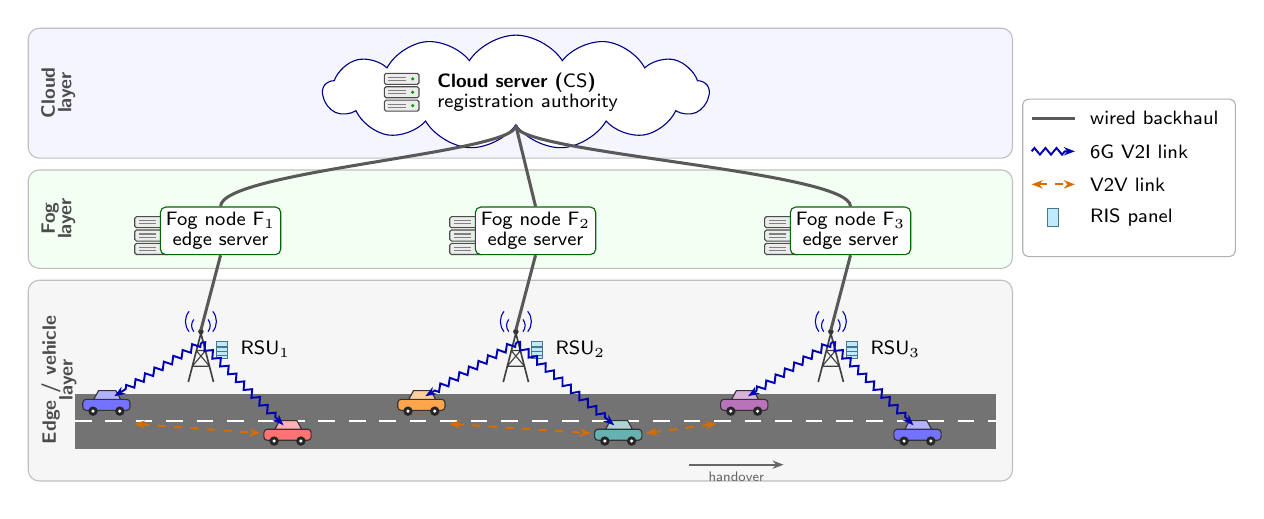
\begin{tikzpicture}[
  font=\sffamily\scriptsize, >={Stealth[length=4pt]},
  wired/.style={line width=1.1pt, draw=black!65},
  air/.style={draw=blue!70!black, line width=0.7pt, decorate, decoration={zigzag, segment length=4pt, amplitude=1.2pt, post length=3pt}, ->},
  v2v/.style={draw=orange!85!black, line width=0.7pt, dashed, <->},
  layer/.style={rounded corners=4pt, draw=black!25, inner sep=0pt, minimum width=12.5cm, anchor=north west},
  ltitle/.style={rotate=90, anchor=north, font=\sffamily\scriptsize\bfseries, text=black!70, align=center},
]
\tikzset{
  server/.pic={
    \foreach \k in {0,1,2}{
      \draw[fill=gray!15, draw=black!70, rounded corners=0.6pt] (-0.22,{0.17*\k}) rectangle (0.22,{0.17*\k+0.14});
      \fill[green!60!black] (0.14,{0.17*\k+0.07}) circle (0.022);
      \draw[black!50] (-0.17,{0.17*\k+0.05}) -- (0.05,{0.17*\k+0.05}) (-0.17,{0.17*\k+0.09}) -- (0.05,{0.17*\k+0.09});
    }
  },
  tower/.pic={
    \draw[black!75, line width=0.6pt] (-0.16,0) -- (0,0.62) -- (0.16,0);
    \draw[black!75] (-0.11,0.2) -- (0.11,0.2) (-0.06,0.4) -- (0.06,0.4) (-0.11,0.2) -- (0.06,0.4) (0.11,0.2) -- (-0.06,0.4);
    \fill[black!80] (0,0.64) circle (0.035);
    \draw[blue!70!black] (0.09,0.64) arc (-40:40:0.12) (0.15,0.64) arc (-40:40:0.2);
    \draw[blue!70!black] (-0.09,0.64) arc (220:140:0.12) (-0.15,0.64) arc (220:140:0.2);
    \draw[fill=cyan!25, draw=cyan!50!black] (0.2,0.3) rectangle (0.34,0.52);
    \foreach \a in {0.335,0.39,0.445} \draw[cyan!50!black] (0.2,\a) -- (0.34,\a);
  },
  pics/car/.style={code={
    \colorlet{carcol}{#1}
    \draw[fill=carcol, draw=black!80, rounded corners=1.2pt] (-0.3,0.06) rectangle (0.3,0.2);
    \draw[fill=carcol!55!white, draw=black!80] (-0.16,0.2) -- (-0.1,0.31) -- (0.12,0.31) -- (0.18,0.2) -- cycle;
    \fill[black!85] (-0.17,0.05) circle (0.06) (0.17,0.05) circle (0.06);
    \fill[white] (-0.17,0.05) circle (0.022) (0.17,0.05) circle (0.022);
  }},
  pics/car/.default=blue!55,
}
% ---------- layers ----------
\begin{scope}[on background layer]
  \node[layer, fill=blue!4,  minimum height=1.65cm] at (0,0) {};
  \node[layer, fill=green!5, minimum height=1.25cm] at (0,-1.8) {};
  \node[layer, fill=gray!7,  minimum height=2.55cm] at (0,-3.2) {};
\end{scope}
\node[ltitle] at (0.05,-0.825) {Cloud\\[-2pt]layer};
\node[ltitle] at (0.05,-2.425) {Fog\\[-2pt]layer};
\node[ltitle] at (0.05,-4.475) {Edge / vehicle\\[-2pt]layer};
% ---------- cloud ----------
\node[cloud, cloud puffs=13, cloud puff arc=115, aspect=3.6, draw=blue!50!black, fill=white, minimum width=4.9cm, minimum height=1.45cm] (cs) at (6.2,-0.82) {};
\pic at ($(cs.center)+(-1.45,-0.24)$) {server};
\node[align=left, font=\sffamily\scriptsize, anchor=west] at ($(cs.center)+(-1.12,0.0)$) {\textbf{Cloud server ($\CS$)}\\[-1pt]registration authority};
% ---------- fog nodes ----------
\foreach \i/\x in {1/2.2,2/6.2,3/10.2}{
  \pic at (\x-0.62,-2.88) {server};
  \node[draw=green!40!black, fill=white, rounded corners=2pt, inner sep=2pt, align=center, font=\sffamily\scriptsize] (f\i) at (\x+0.25,-2.58) {Fog node $\Fog_{\i}$\\[-1pt]edge server};
}
\draw[wired] (cs.south) .. controls +(0,-0.35) and +(0,0.45) .. (f1.north);
\draw[wired] (cs.south) -- (f2.north);
\draw[wired] (cs.south) .. controls +(0,-0.35) and +(0,0.45) .. (f3.north);
% ---------- road ----------
\fill[black!55] (0.6,-5.35) rectangle (12.3,-4.65);
\draw[white, line width=0.8pt, dash pattern=on 6pt off 5pt] (0.6,-5.0) -- (12.3,-5.0);
% ---------- RSUs ----------
\foreach \i/\x in {1/2.2,2/6.2,3/10.2}{
  \pic at (\x,-4.5) {tower};
  \node[font=\sffamily\scriptsize, anchor=west] at (\x+0.38,-4.08) {RSU$_{\i}$};
  \draw[wired] (f\i.south) -- (\x,-3.84);
}
% ---------- vehicles ----------
\pic at (1.0,-4.92) {car=blue!55};
\pic at (3.3,-5.3) {car=red!55};
\pic at (5.0,-4.92) {car=orange!70};
\pic at (7.5,-5.3) {car=teal!60};
\pic at (9.1,-4.92) {car=violet!55};
\pic at (11.3,-5.3) {car=blue!55};
% ---------- links ----------
\draw[air] (2.2,-4.0) -- (1.1,-4.68);
\draw[air] (2.2,-4.0) -- (3.25,-5.05);
\draw[air] (10.2,-4.0) -- (11.25,-5.05);
\draw[v2v] (1.35,-5.03) -- (2.95,-5.15);
\draw[v2v] (7.85,-5.15) -- (8.75,-5.03);
\draw[v2v] (5.35,-5.03) -- (7.15,-5.15);
\draw[air] (6.2,-4.0) -- (5.05,-4.68);
\draw[air] (6.2,-4.0) -- (7.45,-5.05);
\draw[air] (10.2,-4.0) -- (9.15,-4.68);
% ---------- mobility ----------
\draw[-{Stealth[length=4pt]}, black!60, line width=0.8pt] (8.4,-5.55) -- (9.6,-5.55) node[midway, below=-1pt, font=\sffamily\tiny] {handover};
% ---------- legend ----------
\begin{scope}[shift={(12.75,-1.0)}]
  \node[draw=black!30, fill=white, rounded corners=2pt, minimum width=2.7cm, minimum height=2.0cm, anchor=north west] at (-0.12,0.1) {};
  \draw[wired] (0,-0.15) -- (0.55,-0.15); \node[anchor=west] at (0.62,-0.15) {wired backhaul};
  \draw[air] (0,-0.57) -- (0.55,-0.57); \node[anchor=west] at (0.62,-0.57) {6G V2I link};
  \draw[v2v] (0,-0.99) -- (0.55,-0.99); \node[anchor=west] at (0.62,-0.99) {V2V link};
  \draw[fill=cyan!25, draw=cyan!50!black] (0.2,-1.52) rectangle (0.34,-1.30); \node[anchor=west] at (0.62,-1.41) {RIS panel};
\end{scope}
\end{tikzpicture}}
\caption{Architecture of 6G-assisted fog computing within the IoV framework. Vehicles reach fog nodes through 6G roadside units (RSUs) equipped with reconfigurable intelligent surfaces (RIS) and exchange vehicle-to-vehicle (V2V) messages with each other; fog nodes are connected to the cloud server ($\CS$) through a wired backhaul. A moving vehicle hands over from the coverage of one fog node to that of the next.}
\label{fig:arch}
\end{figure*}


\subsection{Motivation and Contributions}
Despite this potential, 6G-vehicular fog computing systems face significant security obstacles \cite{rahdari2025survey}. The scale, dynamics, and heterogeneity of IoV data make secure transmission a critical issue \cite{sutradhar2024survey}, and in vehicular applications a security failure can endanger human lives. Protecting this traffic requires the vehicle, the fog node, and the cloud server to authenticate each other and to agree on session keys.

An important step in this direction was taken in \cite{chen2024provably}, which proposed a protocol to authenticate the vehicle, the fog node, and the cloud server in a single run of four messages and to establish a session key shared by the three. Compared with the earlier three-party schemes for fog-based vehicular networks that use elliptic-curve cryptography (ECC) \cite{ma2019efficient,eftekhari2021security}, this protocol needs fewer point multiplications and transmits fewer bits (Section~\ref{sec:perf}). It also hides the identity of the vehicle and comes with a proof in the real-or-random model. These properties make it attractive for practical deployments. However, we examined the protocol under the Canetti-Krawczyk (CK) adversarial model \cite{canetti2001analysis}, in which the adversary can obtain both long-term and ephemeral secrets. We demonstrated that the protocol remains vulnerable to key escrow, lacks perfect forward secrecy, and is susceptible to ephemeral secret leakage, authentication bypass, and offline password guessing attacks. Moreover, mobility is outside its scope: every authentication requires a round trip to the cloud, and so does each handover between fog nodes.

We propose {\protocol}\footnote{From \emph{fog} and \emph{roaming}: a vehicle roams across fog nodes and authenticates with each of them through bivariate polynomial shares, without contacting the cloud.}, a two-phase authentication protocol based on ECC and bivariate polynomials that addresses these issues. The contributions of this paper are as follows:

\begin{itemize}
    \item We analyze the security of the protocol in \cite{chen2024provably} under the CK adversary and show that it is subject to key escrow, does not provide perfect forward secrecy, and is exposed to ephemeral secret leakage, authentication bypass, and offline password guessing attacks.

    \item We model our cryptanalysis using attack trees with sequential conjunction \cite{jhawar2015attack}, which illustrate the ordered steps by which an adversary exploits each weakness to compromise the session key.

    \item We propose {\protocol}, a two-phase authentication protocol for 6G-assisted fog computing-based IoVs. In the first phase, the vehicle, the fog node, and the cloud server authenticate each other and share a session key with perfect forward secrecy. In the second phase, pairwise keys derived from a bivariate polynomial let a vehicle re-authenticate with any fog node without contacting the cloud; fog nodes keep no per-vehicle state, and handovers become fast.

    \item We prove the semantic security of {\protocol} in the real-or-random model under the CK threat model, and we verify it with the Tamarin prover \cite{meier2013tamarin}. Furthermore, a comprehensive evaluation demonstrates its robustness against various well-known attacks.

    \item We conduct simulations using Veins, SUMO, and OMNeT++ on the road network of Tarragona, Spain, and compare {\protocol} with related works. The results demonstrate its performance in terms of computational cost, communication cost, storage cost, packet loss rate, and latency.
\end{itemize}

\subsection{Organization}
The remainder of this paper is organized as follows. Section~\ref{sec:related} reviews existing authentication protocols for IoV applications. Section~\ref{sec:prelim} introduces the ECC and bivariate polynomial preliminaries and the threat model. Section~\ref{sec:crypt} reviews the protocol in \cite{chen2024provably}, analyzes its security, and models the resulting attacks with attack trees. Section~\ref{sec:proposed} presents {\protocol}. Section~\ref{sec:security} analyzes its security formally, with the Tamarin prover, and informally, and compares it with existing protocols. Section~\ref{sec:perf} evaluates its performance. Finally, Section~\ref{sec:concl} concludes the paper.

\section{Related Work}\label{sec:related}
In recent years, numerous authentication schemes have been proposed for vehicular networks, most of them based on ECC. Conditional privacy-preserving authentication (CPPA) schemes sign every message under a pseudonym: EPA-CPPA \cite{li2018epa} is provably secure and efficient, CPPA-D \cite{xiong2021cppa} keeps messages unforgeable even if the master key or a vehicle key leaks, and the scheme in \cite{wei2020secure} achieves message recovery for traffic emergency messages. However, these schemes establish no session key, so every message requires public-key operations.

The scheme in \cite{yu2018secure} is very lightweight because it uses only hash and XOR operations, but it establishes no session key. The similarly lightweight key agreement in \cite{ahmed2020anonymous} targets vehicle-to-grid interactions. The pairing-free scheme in \cite{cui2020secure} resists side-channel attacks on tamper-proof devices by periodically updating the secrets stored in them, but it requires every vehicle to authenticate with the trusted authority, as does the tree-based key agreement in \cite{wei2021proven}, which secures vehicle-to-vehicle (V2V) and vehicle-to-infrastructure (V2I) communications and supports key updating. The hybrid signcryption protocol in \cite{ali2021ecchsc} provides confidentiality, integrity, and anonymity for heterogeneous V2I communications with low bandwidth but requires public-key operations for every message.

Fog and edge computing have motivated three-party schemes in which a fog node mediates between the vehicle and a cloud or trusted server. The pairing-free key agreement in \cite{ma2019efficient} provides perfect forward secrecy, but its cloud server derives the private keys of all entities from its master key, the leakage of one ephemeral secret exposes the session key \cite{eftekhari2021security}, and it is the most expensive of the compared schemes. AKM-IoV \cite{wazid2019akm} establishes vehicle-fog and fog-cloud keys with hash operations only, but its trusted authority issues all long-term secrets, which also unmask the nonces of past sessions. The pairwise key agreement in \cite{eftekhari2021security} gives each pair of entities a separate key with perfect forward secrecy, but its cloud server derives the long-term credentials of all entities. LBVP \cite{zhang2022lbvp} authenticates vehicles at fog nodes without the online participation of the trusted authority and verifies requests in batches, but its session key depends on ephemeral values only. The certificateless signcryption scheme in \cite{xie2022efficient} avoids pairings and point multiplications in the online phase but protects individual messages rather than establishing session keys.

The protocol in \cite{tian2025provable} supports intra-domain and inter-domain V2V authentication and was evaluated with Veins, SUMO, and OMNeT++, but it addresses V2V communication only. Finally, the protocol of \cite{chen2024provably} represents an important step towards authenticating fog-computing-enabled vehicular networks in a single run through lightweight operations and vehicle identity privacy. However, under the CK adversarial model, we show that this protocol is subject to key escrow, lacks perfect forward secrecy, and is exposed to ephemeral secret leakage, authentication bypass, and offline password guessing attacks (Section~\ref{sec:crypt}). None of these schemes allows a fog node to authenticate a vehicle without the cloud.

\section{Preliminaries}\label{sec:prelim}

\subsection{Elliptic-Curve Cryptography (ECC)}
ECC is a form of public-key cryptography based on the algebraic structure of elliptic curves over finite fields. A non-singular curve $E_p(a,b)$ over the prime field $\mathbb{F}_p$ of integers modulo a prime $p$ is defined by $y^2 = x^3 + ax + b \bmod p$ with $4a^3+27b^2 \not\equiv 0 \pmod p$ \cite{adeniyi2024systematic}. Its points and the point at infinity form a group under point addition; we use a generator $G$ of a subgroup of prime order $n$ and write $k\cdot G$ for scalar multiplication. The security of our construction relies on the following problems \cite{ullah2023elliptic}.
\begin{itemize}
    \item \emph{Elliptic Curve Discrete Logarithm Problem ($\ECDLP$):} given $G$ and $X = x\cdot G$, compute $x\in\mathbb{Z}_n^*=\{1,\dots,n-1\}$.
    \item \emph{Computational Diffie-Hellman Problem ($\CDH$):} given $G$, $x\cdot G$, and $y\cdot G$, compute $xy\cdot G$.
    \item \emph{Gap Diffie-Hellman Problem ($\GDH$):} solve $\CDH$ with access to an oracle that decides whether $(x\cdot G, y\cdot G, Z)$ satisfies $Z = xy\cdot G$.
\end{itemize}
We write $\mathsf{Adv}^{\GDH}(t)$ for the maximum probability with which an algorithm running in time $t$ solves $\GDH$.

\subsection{Bivariate Polynomials and Pairwise Keys}\label{sec:poly}
Let $q$ be a prime and let
\begin{equation}\label{eq:poly}
f(x,y)=\sum_{a=0}^{t_x}\sum_{b=0}^{t_y} c_{a,b}\,x^a y^b \bmod q
\end{equation}
be a bivariate polynomial over the field $\mathbb{F}_q$ of integers modulo $q$, of degree at most $t_x$ in $x$ and at most $t_y$ in $y$. For $u,w\in\mathbb{F}_q$, the univariate polynomials $f(u,y)$ and $f(x,w)$, of degrees at most $t_y$ and $t_x$, are called the \emph{row share} of $u$ and the \emph{column share} of $w$, respectively. The holders of these two shares can both compute the \emph{pairwise key} $f(u,w)$ without interaction, by evaluating their shares at $w$ and at $u$, respectively. A share consists of $t_y+1$ or $t_x+1$ coefficients, and its evaluation with Horner's rule costs $t_y$ or $t_x$ modular multiplications \cite{knuth1997art}. Unlike the symmetric polynomials of \cite{blundo1993perfectly}, $f$ need not satisfy $f(x,y)=f(y,x)$, so a pairwise key is shared only between a row share and a column share, and the degrees $t_x$ and $t_y$ can be chosen independently. The following lemma shows that $f(u,w)$ remains secret even if up to $t_x$ other row shares and $t_y$ other column shares are known.

\begin{lemma}\label{lem:poly}
Let $f$ be a polynomial of the form \eqref{eq:poly} whose coefficients $c_{a,b}$ are independent and uniformly distributed in $\mathbb{F}_q$, with $q>\max(t_x,t_y)$. Let $X,Y\subset\mathbb{F}_q$ with cardinalities $|X|\le t_x$ and $|Y|\le t_y$, and let $u\in\mathbb{F}_q\setminus X$ and $w\in\mathbb{F}_q\setminus Y$. Then $f(u,w)$ is uniformly distributed in $\mathbb{F}_q$ and independent of the univariate polynomials $f(a,y)$ for $a\in X$ and $f(x,b)$ for $b\in Y$.
\end{lemma}
\begin{proof}
Since $q>\max(t_x,t_y)$, there exist sets $X'\supseteq X\cup\{u\}$ and $Y'\supseteq Y\cup\{w\}$ of exactly $t_x+1$ and $t_y+1$ elements of $\mathbb{F}_q$, respectively. The map from the coefficients $(c_{a,b})$ to the values $(f(\alpha,\beta))_{\alpha\in X',\beta\in Y'}$ is linear, and its matrix is the Kronecker product $V_{X'}\otimes V_{Y'}$ of the Vandermonde matrices of $X'$ and $Y'$, which are invertible because their nodes are distinct. Hence, this map is a bijection, and the $(t_x+1)(t_y+1)$ values of $f$ on the grid $X'\times Y'$ are independent and uniformly distributed. For $a\in X$, the polynomial $f(a,y)$ has degree at most $t_y$ and is therefore determined, by Lagrange interpolation, by its values on $\{a\}\times Y'$; likewise, $f(x,b)$ for $b\in Y$ is determined by its values on $X'\times\{b\}$. All these polynomials are thus functions of the grid values on $(X\times Y')\cup(X'\times Y)$, which does not contain $(u,w)$ because $u\notin X$ and $w\notin Y$. Since $f(u,w)$ is itself a grid value, it is uniform and independent of them.
\end{proof}

\subsection{Threat Model}\label{sec:threat}
We consider the Canetti-Krawczyk (CK) threat model \cite{canetti2001analysis}. Its adversary $\Adv$ is more powerful than that of the Dolev-Yao model \cite{dolev1983security}, and the protocol must ensure that leaked long-term private keys or ephemeral secrets do not compromise the security of other sessions.
\begin{itemize}
    \item \emph{Adversary's goal:} $\Adv$ aims to learn a session key, to make an honest party accept a session with a partner that did not take part in it, or to learn or trace the identity of an anonymous party.
    \item \emph{Adversary's knowledge:} $\Adv$ knows all public information, such as public keys, identities, domain parameters, and the protocol specification; the primitives are ideal, so it cannot invert hash functions, find collisions, or decrypt without the key.
    \item \emph{Adversary's capabilities:} $\Adv$ controls the public channel: it can intercept, inject, modify, delete, replay, concatenate, or split messages, and it can initiate sessions with legitimate parties, possibly with compromised credentials. It can learn previous session keys, the ephemeral secrets of any session, and the long-term secrets of every party including the trusted servers. It can also capture the device of a party and read its memory, but then does not know the password that protects the stored credentials. To exclude trivial attacks, $\Adv$ may not learn both the long-term secret and the ephemeral secret of the same party in the session under attack, and it may not corrupt a partner of that session before the session completes.
\end{itemize}

\section{Cryptanalysis of the Protocol in \texorpdfstring{\cite{chen2024provably}}{[11]}}\label{sec:crypt}
The protocol in \cite{chen2024provably} involves three entities, the vehicle $\Veh_i$, the fog node $\Fog_j$, and the cloud server $\CS$, and runs in two phases: registration and mutual authentication. We first review both phases in the notation of \cite{chen2024provably} and then examine its security and model the resulting attacks with attack trees.

\subsection{Review of the Protocol}
\emph{Registration phase:} $\Veh_i$ and $\Fog_j$ register with $\CS$ through a secure channel. $\Veh_i$ chooses its identity $\VID_i$, its password $\VPW_i$, and a random number $r_1$, computes $\PV_i=\h(\VID_i\cat\VPW_i\cat r_1)$, where $\h(\cdot)$ is a hash function and $\cat$ denotes concatenation, and sends $\{\VID_i,\PV_i\}$ to $\CS$. Using its master secret $K_c$, $\CS$ computes the private key $a_i=\h(\VID_i\cat\PV_i\cat K_c)$ of $\Veh_i$, the public key $A_i=a_i\cdot G$, and $\MV_i=a_i\oplus\PV_i$, with $\oplus$ the bitwise XOR, which it returns to $\Veh_i$. $\Veh_i$ computes $\TV_i=\h(\VID_i\oplus\VPW_i\cat a_i)$ and stores $\{\TV_i,\MV_i,r_1\}$. Similarly, $\Fog_j$ sends its identity $\FID_j$ to $\CS$, which picks a random $r_2$ and computes $\PFD_j=\h(\FID_j\cat r_2)$, the private key $b_j=\h(\PFD_j\cat K_c)$ of $\Fog_j$, its public key $B_j=b_j\cdot G$, and the shared key $K_{cf}=\h(\FID_j\oplus K_c)$. $\CS$ stores $\FID_j$ and sends $\{\PFD_j,b_j,K_{cf}\}$ to $\Fog_j$, which stores $\Rb_j=b_j\oplus\h(\FID_j\cat K_{cf})$, $\PFD_j$, and $\RK_{cf}=K_{cf}\oplus\FID_j$.

\emph{Mutual authentication phase:} The messages $M_1$ to $M_4$ and the computation of the session key $\SK$ are summarized in Fig.~\ref{fig:chen}. The identity $\FID_j$ and the public key $B_j$ of a fog node are public, since every vehicle needs them to compute $M_1$.

\begin{figure*}[!t]
\centering
\scalebox{0.82}{%
\begin{msc}{}
  \setmsckeyword{}
  % per element: \mscact[extra levels][box width]{instance}{...}, \mscmess[trim at sender][trim at receiver]{label}{from}{to}
  \drawframe{no}
  \setlength{\instwidth}{2.7cm}
  \setlength{\instdist}{2.8cm}
  \setlength{\envinstdist}{2.6cm}
  \setlength{\levelheight}{0.4cm}
  \setlength{\topheaddist}{0.1cm}
  \setlength{\firstlevelheight}{0.25cm}
  \setlength{\lastlevelheight}{0.25cm}
  \declinst{v}{}{\textbf{Vehicle} $\Veh_i$}
  \declinst{f}{}{\textbf{Fog node} $\Fog_j$}
  \declinst{c}{}{\textbf{Cloud server} $\CS$}
  % ---- V_i ----
  \mscact[1.6][3.8cm]{v}{%
    Input $\VID_i^*, \VPW_i^*$\\
    $\PV_i=\h(\VID_i^*\cat\VPW_i^*\cat r_1)$\\
    $a_i=\MV_i\oplus\PV_i$\\
    $\TV_i^*=\h(\VID_i^*\oplus\VPW_i^*\cat a_i)$\\
    Verify $\TV_i^*\chk\TV_i$\\
    Generate $r_3, r_3', T_1$\\
    $P_i=r_3\cdot G$\\
    $Q_i=r_3\cdot B_j$\\
    $F_i=r_3'\oplus Q_i$\\
    $\RID_i=\VID_i\oplus(Q_i\oplus\FID_j)$}
  \mscmess[0cm][0cm]{\footnotesize $M_1=\{\RID_i, P_i, F_i, T_1\}$}{v}{f}
  \nextlevel[0.5]
  % ---- F_j ----
  \mscact[1.6][4.35cm]{f}{%
    Verify $|T_1-T_c|\le\Delta T$\\
    $K_{cf}=\RK_{cf}\oplus\FID_j$\\
    $b_j=\Rb_j\oplus\h(\FID_j\cat K_{cf})$\\
    $Q_i=b_j\cdot P_i$\\
    $r_3'=F_i\oplus Q_i$\\
    $R_i=\RID_i\oplus Q_i$\\
    Generate $r_4, T_2$\\
    $W_i=r_4\oplus\h(K_{cf}\cat\FID_j)$\\
    $Y_i=R_i\oplus\h(K_{cf}\oplus r_4)$\\
    $X_i=\PFD_j\oplus\h(\FID_j\cat K_{cf}\oplus r_4)$\\
    $D=\h(\PFD_j\cat r_4\cat R_i\oplus K_{cf})$}
  \mscmess[0cm][0cm]{\footnotesize $M_2=\{W_i, X_i, Y_i, D, T_2\}$}{f}{c}
  \nextlevel[0.5]
  % ---- CS ----
  \mscact[1.6][4.75cm]{c}{%
    Verify $|T_2-T_c|\le\Delta T$\\
    $K_{cf}=\h(\FID_j\oplus K_c)$\\
    $r_4^*=W_i\oplus\h(K_{cf}\cat\FID_j)$\\
    $R_i^*=Y_i\oplus\h(K_{cf}\oplus r_4^*)$\\
    $\PFD_j^*=X_i\oplus\h(\FID_j\cat K_{cf}\oplus r_4^*)$\\
    Verify $\h(\PFD_j^*\cat r_4^*\cat R_i^*\oplus K_{cf})\chk D$\\
    Generate $r_5, T_3$\\
    $\SK=\h(\PFD_j\cat R_i\cat r_4\cat r_5\oplus K_{cf})$\\
    $Z_i=\h(\SK\cat K_{cf}\oplus\FID_j)$\\
    $L_i=r_5\oplus\h(K_{cf}\oplus\FID_j\cat r_4)$}
  \mscmess[0cm][0cm]{\footnotesize $M_3=\{L_i, Z_i, T_3\}$}{c}{f}
  \nextlevel[0.5]
  % ---- F_j ----
  \mscact[1.6][4.7cm]{f}{%
    Verify $|T_3-T_c|\le\Delta T$\\
    $r_5^*=L_i\oplus\h(K_{cf}\oplus\FID_j\cat r_4)$\\
    $\SK^*=\h(\PFD_j\cat R_i\cat r_4\cat r_5^*\oplus K_{cf})$\\
    Verify $\h(\SK^*\cat K_{cf}\oplus\FID_j)\chk Z_i$\\
    Generate $T_4$\\
    $J_i=\h(\RID_i\cat r_3'\oplus Q_i)$\\
    $N_i=\h(\FID_j\oplus Q_i\cat R_i)\oplus\SK$}
  \mscmess[0cm][0cm]{\footnotesize $M_4=\{N_i, J_i, T_4\}$}{f}{v}
  \nextlevel[0.5]
  % ---- V_i ----
  \mscact[0.4][5.1cm]{v}{%
    Verify $|T_4-T_c|\le\Delta T$\\
    Verify $\h(\RID_i\cat r_3'\oplus Q_i)\chk J_i$\\
    $\SK=N_i\oplus\h(\FID_j\oplus Q_i\cat\VID_i\oplus\FID_j)$}
\end{msc}}
\caption{Mutual authentication phase of the protocol in \cite{chen2024provably}.}
\label{fig:chen}
\end{figure*}


\subsection{Weaknesses}\label{sec:weak}

\emph{1) Key escrow and master-key exposure:} To avoid key escrow, private keys are usually generated by their owners, so that no third party holds them, not even a trusted one. In \cite{chen2024provably}, $\CS$ generates the private keys $a_i$ and $b_j$ of all vehicles and fog nodes, and every session key depends on the master secret $K_c$. Since $\FID_j$ is public, an adversary that learns $K_c$ computes $K_{cf}=\h(\FID_j\oplus K_c)$ and, from the recorded messages $M_2$ and $M_3$ of any past or future session, recovers $r_4=W_i\oplus\h(K_{cf}\cat\FID_j)$, $\PFD_j=X_i\oplus\h(\FID_j\cat K_{cf}\oplus r_4)$, $R_i=Y_i\oplus\h(K_{cf}\oplus r_4)$, and $r_5=L_i\oplus\h(K_{cf}\oplus\FID_j\cat r_4)$, and hence $\SK=\h(\PFD_j\cat R_i\cat r_4\cat r_5\oplus K_{cf})$. It also obtains $b_j=\h(\PFD_j\cat K_c)$. Thus $K_c$ is a single point of failure for all sessions in the system, and neither ephemeral values nor the keys of the vehicle protect them.

\emph{2) Lack of perfect forward secrecy:} Perfect forward secrecy requires that the compromise of long-term keys does not reveal past session keys. In this protocol, the session key is recovered by $\Veh_i$ as $\SK=N_i\oplus\h(\FID_j\oplus Q_i\cat\VID_i\oplus\FID_j)$, where $Q_i=r_3\cdot B_j=b_j\cdot P_i$ and $\VID_i\oplus\FID_j=R_i=\RID_i\oplus Q_i$. Hence, an adversary that compromises $\Fog_j$ and obtains $b_j=\Rb_j\oplus\h(\FID_j\cat\RK_{cf}\oplus\FID_j)$ computes $Q_i=b_j\cdot P_i$ from the recorded $P_i$, then $R_i$, and finally $\SK$ for every past session of $\Fog_j$. As in weakness~1, the same holds for $K_{cf}$, which $\Fog_j$ also stores. The session key thus depends on a single static-ephemeral Diffie-Hellman value, and the contribution of $\Fog_j$ is not randomized.

\emph{3) Ephemeral secret leakage:} Under the CK model, the ephemeral secrets of a session may leak through side channels or a weak random number generator, and this leakage should not reveal its session key. Here, $Q_i$ is computed by $\Veh_i$ as $r_3\cdot B_j$, where $B_j$ is public. An adversary that learns $r_3$ therefore computes $Q_i$, $R_i=\RID_i\oplus Q_i$, and $\SK=N_i\oplus\h(\FID_j\oplus Q_i\cat R_i)$ from the public messages $M_1$ and $M_4$.

\emph{4) Authentication bypass:} The private key $a_i$ of $\Veh_i$ is used only to verify the password locally, and no message of the authentication phase depends on a secret of $\Veh_i$. Moreover, neither $\Fog_j$ nor $\CS$ keeps a list of valid vehicle identities. An unregistered adversary can therefore pick any identity $\VID_a$ and random values $r_3,r_3'$, compute $P_i=r_3\cdot G$, $Q_i=r_3\cdot B_j$, $\RID_i=\VID_a\oplus Q_i\oplus\FID_j$, and $F_i=r_3'\oplus Q_i$ from the public key $B_j$, and send $M_1=\{\RID_i,P_i,F_i,T_1\}$ to $\Fog_j$. Both $\Fog_j$ and $\CS$ accept, and $\Fog_j$ returns $M_4$, from which the adversary computes $\SK=N_i\oplus\h(\FID_j\oplus Q_i\cat\VID_a\oplus\FID_j)$. The adversary thus establishes an authenticated session key with $\Fog_j$ and $\CS$ under an arbitrary identity. The authentication fails in the other direction as well: the value $J_i=\h(\RID_i\cat r_3'\oplus Q_i)$ that $\Veh_i$ uses to authenticate $\Fog_j$ equals $\h(\RID_i\cat F_i)$ and can be computed by anyone from $M_1$.

\emph{5) Offline password guessing:} An adversary that captures the on-board unit (OBU) of $\Veh_i$ reads $\{\TV_i,\MV_i,r_1\}$ and verifies guesses $(\VID_i^*,\VPW_i^*)$ offline by checking $\h(\VID_i^*\oplus\VPW_i^*\cat\MV_i\oplus\h(\VID_i^*\cat\VPW_i^*\cat r_1))\chk\TV_i$. A correct guess reveals the identity and the password of $\Veh_i$, so the adversary can log in as $\Veh_i$ and obtain the session keys of the sessions that it runs in the name of $\Veh_i$. The adversary must guess the identity and the password jointly, but both have low entropy. With a single GPU, about $10^{12}$ pairs can be tried within a few minutes. As a try, we implemented this attack with a simple Python~3.13 script on one core of a 2-core virtual machine with an Intel Xeon processor at 2.10~GHz and 8~GB of RAM, using SHA-1 as $\h(\cdot)$. Among 2000 identities and 5000 passwords, i.e., $10^7$ guesses, the script found exactly one matching pair in 42~s, and this pair was the correct one. It also recovered the private key $a_i=\MV_i\oplus\PV_i$ correctly.

\subsection{Modeling the Cryptanalysis via Attack Trees}\label{sec:at}
Attack trees \cite{schneier1999attack} and their extension with sequential conjunction \cite{jhawar2015attack,gadyatskaya2017refinement} represent attacks against a system in a structured and hierarchical manner. The root node represents the ultimate goal of the attacker, and the children of a node refine it into sub-goals. A refinement is disjunctive (\texttt{OR}), conjunctive (\texttt{AND}), or sequentially conjunctive (\texttt{SAND}): \texttt{OR} requires one of the sub-goals, \texttt{AND} requires all sub-goals in any order, and \texttt{SAND} requires all sub-goals in the given order \cite{kordy2014attack}. The leaves are the basic actions of the attacker, and the semantics of a tree is given by sets of series-parallel graphs, which capture the order constraints imposed by \texttt{SAND} \cite{jhawar2015attack}.

We take as root goal the compromise of the session key $\SK$ and define the following basic actions according to Section~\ref{sec:weak}: $\mathit{corCS}$, corrupt $\CS$ and obtain $K_c$; $\mathit{corFN}$, corrupt $\Fog_j$ and obtain $b_j$; $\mathit{esv}$, reveal the ephemeral secret $r_3$; $\mathit{exe}$, eavesdrop the messages of the session; $\mathit{calcKcf}$, compute $K_{cf}$ and unmask $r_4$, $\PFD_j$, $R_i$, and $r_5$ from $M_2$ and $M_3$; $\mathit{calcQb}$ and $\mathit{calcQr}$, compute $Q_i=b_j\cdot P_i$ and $Q_i=r_3\cdot B_j$, respectively, together with $R_i=\RID_i\oplus Q_i$; $\mathit{forge}$, build $M_1$ for an arbitrary identity from $B_j$; $\mathit{snd}$ and $\mathit{rcv}$, send $M_1$ to $\Fog_j$ and receive $M_4$; $\mathit{dSK}_K$ and $\mathit{dSK}_Q$, derive $\SK$ from the unmasked values and from $(N_i,Q_i,R_i)$, respectively; $\mathit{cap}$, capture the on-board unit of $\Veh_i$ and read $\{\TV_i,\MV_i,r_1\}$; $\mathit{guess}$, find $(\VID_i,\VPW_i)$ offline; and $\mathit{run}$, log in as $\Veh_i$ and run the protocol, which yields $\SK$. The resulting tree is shown in Fig.~\ref{fig:attacktree}. Its five branches (A) to (E) correspond to weaknesses~1 to~5. Corruption and eavesdropping are combined with \texttt{AND} because the transcript may be recorded before or after the corruption, which is precisely the lack of forward secrecy; the remaining steps must follow in order and are therefore combined with \texttt{SAND}. Branch~(D) needs neither corruption nor registration, which makes it the cheapest attack. Branch~(E) requires the physical capture of a vehicle but gives the adversary the identity of a legitimate vehicle.

\begin{figure*}[!t]
\centering
\resizebox{\textwidth}{!}{%
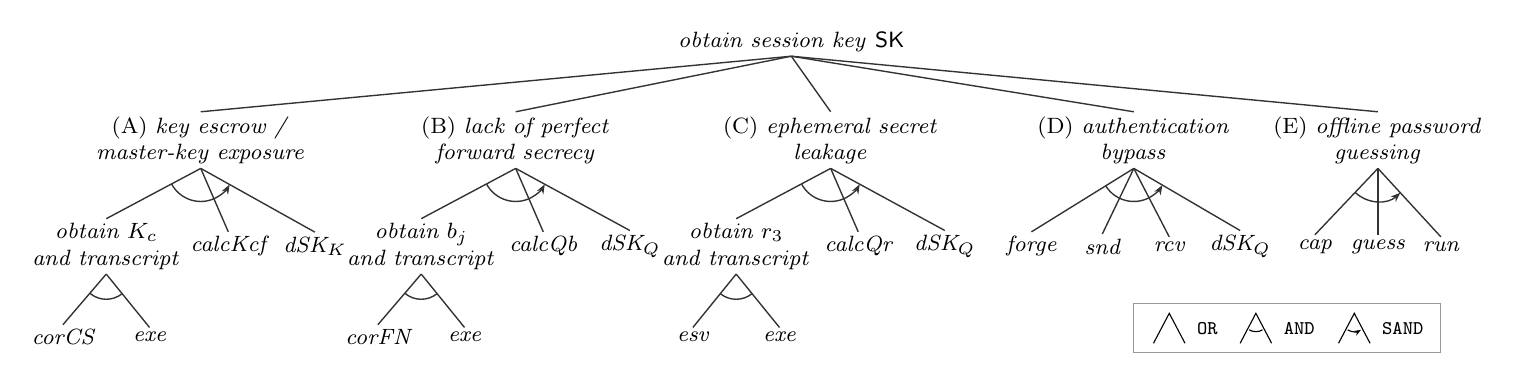
\begin{tikzpicture}[
  font=\footnotesize,
  nd/.style={inner sep=1.5pt, align=center},
  lf/.style={inner sep=1.5pt, align=center, font=\footnotesize\itshape},
  edge/.style={draw=black!80, line width=0.5pt},
]
% ---------- helpers: refinement arcs ----------
\newcommand{\refarc}[5][]{% [arrow] parent, first child, last child, radius
  \draw[black!80, line width=0.5pt, #1] let \p0=(#2.south), \p1=($(#3.north)-(\p0)$), \p2=($(#4.north)-(\p0)$),
    \n1={atan2(\y1,\x1)}, \n2={atan2(\y2,\x2)} in
    ($(\p0)+(\n1:#5)$) arc[start angle=\n1, end angle=\n2, radius=#5];}
\newcommand{\andarc}[4]{\refarc{#1}{#2}{#3}{#4}}
\newcommand{\sandarc}[4]{\refarc[-{Stealth[length=3.5pt]}]{#1}{#2}{#3}{#4}}
% ---------- nodes ----------
\node[nd] (root) at (9.4,0) {\textit{obtain session key} $\SK$};
\node[nd] (A) at (1.9,-1.25) {(A) \textit{key escrow /}\\\textit{master-key exposure}};
\node[nd] (B) at (5.9,-1.25) {(B) \textit{lack of perfect}\\\textit{forward secrecy}};
\node[nd] (C) at (9.9,-1.25) {(C) \textit{ephemeral secret}\\\textit{leakage}};
\node[nd] (D) at (13.75,-1.25) {(D) \textit{authentication}\\\textit{bypass}};
\node[nd] (E) at (16.85,-1.25) {(E) \textit{offline password}\\\textit{guessing}};
% (A)
\node[nd] (A1) at (0.7,-2.6) {\textit{obtain $K_c$}\\\textit{and transcript}};
\node[lf] (A2) at (2.25,-2.6) {calcKcf};
\node[lf] (A3) at (3.35,-2.6) {dSK$_K$};
\node[lf] (A11) at (0.15,-3.75) {corCS};
\node[lf] (A12) at (1.25,-3.75) {exe};
% (B)
\node[nd] (B1) at (4.7,-2.6) {\textit{obtain $b_j$}\\\textit{and transcript}};
\node[lf] (B2) at (6.25,-2.6) {calcQb};
\node[lf] (B3) at (7.35,-2.6) {dSK$_Q$};
\node[lf] (B11) at (4.15,-3.75) {corFN};
\node[lf] (B12) at (5.25,-3.75) {exe};
% (C)
\node[nd] (C1) at (8.7,-2.6) {\textit{obtain $r_3$}\\\textit{and transcript}};
\node[lf] (C2) at (10.25,-2.6) {calcQr};
\node[lf] (C3) at (11.35,-2.6) {dSK$_Q$};
\node[lf] (C11) at (8.15,-3.75) {esv};
\node[lf] (C12) at (9.25,-3.75) {exe};
% (D)
\node[lf] (D1) at (12.45,-2.6) {forge};
\node[lf] (D2) at (13.35,-2.6) {snd};
\node[lf] (D3) at (14.2,-2.6) {rcv};
\node[lf] (D4) at (15.1,-2.6) {dSK$_Q$};
% (E)
\node[lf] (E1) at (16.05,-2.6) {cap};
\node[lf] (E2) at (16.85,-2.6) {guess};
\node[lf] (E3) at (17.65,-2.6) {run};
% ---------- edges ----------
\foreach \c in {A,B,C,D,E} \draw[edge] (root.south) -- (\c.north);
\foreach \c in {A1,A2,A3} \draw[edge] (A.south) -- (\c.north);
\foreach \c in {A11,A12} \draw[edge] (A1.south) -- (\c.north);
\foreach \c in {B1,B2,B3} \draw[edge] (B.south) -- (\c.north);
\foreach \c in {B11,B12} \draw[edge] (B1.south) -- (\c.north);
\foreach \c in {C1,C2,C3} \draw[edge] (C.south) -- (\c.north);
\foreach \c in {C11,C12} \draw[edge] (C1.south) -- (\c.north);
\foreach \c in {D1,D2,D3,D4} \draw[edge] (D.south) -- (\c.north);
\foreach \c in {E1,E2,E3} \draw[edge] (E.south) -- (\c.north);
% ---------- refinements ----------
\sandarc{A}{A1}{A3}{0.42cm}
\sandarc{B}{B1}{B3}{0.42cm}
\sandarc{C}{C1}{C3}{0.42cm}
\sandarc{D}{D1}{D4}{0.42cm}
\sandarc{E}{E1}{E3}{0.42cm}
\andarc{A1}{A11}{A12}{0.32cm}
\andarc{B1}{B11}{B12}{0.32cm}
\andarc{C1}{C11}{C12}{0.32cm}
% ---------- legend ----------
\begin{scope}[shift={(13.75,-3.95)}]
  \draw[black!40] (0,0) rectangle (3.9,0.62);
  \draw (0.25,0.12) -- (0.45,0.5) -- (0.65,0.12); \node[anchor=west, font=\scriptsize\ttfamily] at (0.68,0.3) {OR};
  \draw (1.35,0.12) -- (1.55,0.5) -- (1.75,0.12); \draw (1.465,0.29) arc[start angle=240, end angle=300, radius=0.17];
  \node[anchor=west, font=\scriptsize\ttfamily] at (1.78,0.3) {AND};
  \draw (2.6,0.12) -- (2.8,0.5) -- (3.0,0.12); \draw[-{Stealth[length=2.5pt]}] (2.715,0.29) arc[start angle=240, end angle=300, radius=0.17];
  \node[anchor=west, font=\scriptsize\ttfamily] at (3.03,0.3) {SAND};
\end{scope}
\end{tikzpicture}}
\caption{Attack tree that models the cryptanalysis of the protocol in~\cite{chen2024provably}. Basic actions: $\mathit{corCS}$, corrupt $\CS$ and obtain its master secret $K_c$; $\mathit{corFN}$, corrupt $\Fog_j$ and obtain its private key $b_j$; $\mathit{esv}$, reveal the ephemeral secret $r_3$ of $\Veh_i$; $\mathit{exe}$, eavesdrop the messages of the session; $\mathit{calcKcf}$, compute $K_{cf}$ and unmask $r_4$, $\PFD_j$, $R_i$, and $r_5$ from $M_2$ and $M_3$; $\mathit{calcQb}$ and $\mathit{calcQr}$, compute $Q_i=b_j\cdot P_i$ and $Q_i=r_3\cdot B_j$, respectively, and $R_i=\RID_i\oplus Q_i$; $\mathit{forge}$, build $M_1$ for an arbitrary identity from $B_j$; $\mathit{snd}$ and $\mathit{rcv}$, send $M_1$ to $\Fog_j$ and receive $M_4$; $\mathit{dSK}_K$ and $\mathit{dSK}_Q$, derive $\SK$ from the unmasked values and from $(N_i,Q_i,R_i)$, respectively; $\mathit{cap}$, capture the on-board unit of $\Veh_i$ and read $\{\TV_i,\MV_i,r_1\}$; $\mathit{guess}$, find $(\VID_i,\VPW_i)$ offline; $\mathit{run}$, log in as $\Veh_i$ and run the protocol.}
\label{fig:attacktree}
\end{figure*}


\section{Proposed Protocol}\label{sec:proposed}
We now present {\protocol}, our authentication protocol for the 6G-assisted fog-based IoV of Fig.~\ref{fig:arch}. It consists of a registration phase and two authentication phases. Phase~$\mathsf{A}$ involves the cloud server and runs when a vehicle joins the system or must be re-validated by $\CS$. Phase~$\mathsf{B}$ runs between a vehicle and a fog node only, for example when the vehicle hands over to another fog node. Table~\ref{tab:notation} summarizes the notation.

\begin{table}[!t]
\centering
\caption{Notation of {\protocol}}
\label{tab:notation}
\footnotesize
\renewcommand{\arraystretch}{1.1}
\scalebox{0.9}{%
\begin{tabular}{@{}l p{5.6cm}@{}}
\toprule
\textbf{Notation} & \textbf{Definition}\\
\midrule
$\Veh_i$, $\Fog_j$, $\CS$ & $i$-th vehicle, $j$-th fog node, cloud server\\
$\VID_i$, $\VPW_i$ & Identity and password of $\Veh_i$\\
$\FID_j$ & Identity of $\Fog_j$\\
$\sk_i$, $\pk_i$ & Private and public keys of $\Veh_i$\\
$\sk_j$, $\pk_j$; $\sk_c$, $\pk_c$ & Key pairs of $\Fog_j$ and $\CS$\\
$k_{ic}$, $k_{jc}$ & Static keys $\h(\sk_i\cdot\pk_c)$ and $\h(\sk_j\cdot\pk_c)$\\
$f(x,y)$; $t_x$, $t_y$ & Bivariate polynomial; its degrees in $x$ and $y$\\
$\psi_i(y)$, $\varphi_j(x)$ & Shares $f(\VID_i,y)$ of $\Veh_i$ and $f(x,\FID_j)$ of $\Fog_j$\\
$k_{ij}$ & Pairwise key $f(\VID_i,\FID_j)$ of $\Veh_i$ and $\Fog_j$\\
$r_\ell$, $x_\ell$, $R_\ell$ & Ephemeral secret, scalar $\hT{x}(r_\ell\cat\sk)$, point $x_\ell\cdot G$\\
$\h(\cdot)$, $\Enc/\Dec$ & Hash function, symmetric encryption/decryption\\
$\SK$, $\SK'$ & Session keys of phase $\mathsf{A}$ and phase $\mathsf{B}$\\
$T_\ell$, $\Delta T$ & Timestamps and maximum transmission delay\\
$\RL$ & Revocation list of vehicle identities\\
$\oplus$, $\|$ & XOR and concatenation\\
\bottomrule
\end{tabular}}
\end{table}

\subsection{Design Rationale}\label{sec:rationale}
{\protocol} retains the three-party architecture of \cite{chen2024provably} and addresses each weakness of Section~\ref{sec:weak} with a dedicated element of the design; element~(iv) adds cloud-free authentication.

\emph{(i) No key escrow (weakness~1).} Every entity generates its own key pair; $\CS$ never learns $\sk_i$ or $\sk_j$.

\emph{(ii) Forward secrecy and ephemeral secret leakage (weaknesses~2 and~3).} The ephemeral scalar of each session is $x=\hT{x}(r\cat\sk)$, so that it remains secret unless both the ephemeral secret $r$ and the long-term key $\sk$ of the same entity leak; every session key additionally depends on an ephemeral-ephemeral Diffie-Hellman value, so that the later compromise of all long-term keys does not reveal it.

\emph{(iii) Authentication against the cloud (weakness~4).} The vehicle authenticates to $\CS$ with a tag under $k_{ic}$ that the fog node cannot compute, and the fog node authenticates to $\CS$ with a key derived from $k_{jc}$; this rules out authentication bypass and impersonation of vehicles by a compromised fog node.

\emph{(iv) Offline password guessing (weakness~5).} The vehicle stores only a fuzzy verifier of its password and keeps its credentials under an unauthenticated encryption, so that a captured on-board unit does not allow an offline check of password guesses.

\emph{(v) Cloud-free authentication by fog nodes.} A fog node must authenticate \emph{any} registered vehicle, including ones registered after its deployment, without contacting $\CS$ or storing per-vehicle data: per-vehicle keys cost storage linear in the number of vehicles plus an update at every registration and revocation, certificates cost about two point multiplications per verification, and a $\CS$ query adds the backhaul round trip that handovers must avoid. Encoding identities as elements of $\mathbb{F}_q$ (Section~\ref{sec:poly}) and giving each vehicle and fog node the row and column share of its identity provides every vehicle-fog pair with a key $k_{ij}$ at $t_x$ modular multiplications and constant storage; this makes phase~$\mathsf{B}$ possible and lets the fog reject forged requests before involving $\CS$. By Lemma~\ref{lem:poly}, up to $t_x$ vehicle and $t_y$ fog shares reveal nothing about any other pair, so we set $t_y$ to the number of fog nodes and $t_x$ to the on-board units capturable within one epoch, after which $f$ is renewed (Section~\ref{sec:revocation}). As session keys always include Diffie-Hellman values, even a reconstructed $f$ enables only phase-$\mathsf{B}$ impersonation, never session-key recovery.

\subsection{System Setup and Registration}
$\CS$ selects a non-singular curve $E_p(a,b)$ with a generator $G$ of prime order $n$, a hash function $\h:\{0,1\}^*\rightarrow\{0,1\}^l$, written $\hT{t}(m)=\h(\mathsf{t}\cat m)$ when its input starts with the constant domain-separation tag $\mathsf{t}$, and a symmetric cipher in counter mode with encryption function $\Enc$ and decryption function $\Dec$. It generates its key pair $\sk_c\in\mathbb{Z}_n^*$ and $\pk_c=\sk_c\cdot G$, selects the polynomial $f$ of the current epoch according to \eqref{eq:poly}, and publishes $\{E_p(a,b),G,n,\h,\Enc,\Dec,\pk_c\}$.

\emph{Fog node registration:} $\Fog_j$ chooses $\FID_j$, generates $\sk_j\in\mathbb{Z}_n^*$ and $\pk_j=\sk_j\cdot G$, and sends $\{\FID_j,\pk_j\}$ to $\CS$ over a secure channel. $\CS$ returns the share $\varphi_j(x)=f(x,\FID_j)$ and the current revocation list ($\RL$), and both parties compute the static key $k_{jc}=\h(\sk_j\cdot\pk_c)=\h(\sk_c\cdot\pk_j)$. $\CS$ stores $\{\FID_j,\pk_j,k_{jc}\}$, and $\Fog_j$ stores $\{\sk_j,k_{jc},\varphi_j,\RL\}$.

\emph{Vehicle registration:} $\Veh_i$ chooses $\VID_i$, $\VPW_i$, and a random $b_i$, generates $\sk_i\in\mathbb{Z}_n^*$ and $\pk_i=\sk_i\cdot G$, and sends $\{\VID_i,\pk_i\}$ to $\CS$ over a secure channel. $\CS$ returns the share $\psi_i(y)=f(\VID_i,y)$ and the directory $\{(\FID_j,\pk_j)\}$ of the fog nodes, and both parties compute $k_{ic}=\h(\sk_i\cdot\pk_c)=\h(\sk_c\cdot\pk_i)$. $\CS$ stores $\{\VID_i,\pk_i,k_{ic}\}$. $\Veh_i$ computes $\HPW_i=\h(\VID_i\cat\VPW_i\cat b_i)$, the fuzzy verifier $\TV_i=\h(\HPW_i)\bmod n_0$ with $2^4\le n_0\le 2^8$, and $\Cred_i=\Enc_{\HPW_i}(\sk_i\cat k_{ic}\cat\psi_i)$; it stores $\{b_i,\TV_i,\Cred_i\}$ with the public directory and erases the other values.

\begin{figure*}[!t]
\centering
\scalebox{0.82}{%
\begin{msc}{}
  \setmsckeyword{}
  % per element: \mscact[extra levels][box width]{instance}{...}, \mscmess[trim at sender][trim at receiver]{label}{from}{to}
  \drawframe{no}
  \setlength{\instwidth}{2.7cm}
  \setlength{\instdist}{2.8cm}
  \setlength{\envinstdist}{2.6cm}
  \setlength{\levelheight}{0.4cm}
  \setlength{\topheaddist}{0.1cm}
  \setlength{\firstlevelheight}{0.25cm}
  \setlength{\lastlevelheight}{0.25cm}
  \declinst{v}{}{\textbf{Vehicle} $\Veh_i$}
  \declinst{f}{}{\textbf{Fog node} $\Fog_j$}
  \declinst{c}{}{\textbf{Cloud server} $\CS$}
  % ---- Step 1: V_i ----
  \mscact[1.6][4.5cm]{v}{%
    Input $\VID_i^*, \VPW_i^*$\\
    $\HPW_i^*=\h(\VID_i^*\cat\VPW_i^*\cat b_i)$\\
    Verify $\h(\HPW_i^*)\bmod n_0\chk\TV_i$\\
    $(\sk_i\cat k_{ic}\cat\psi_i)=\Dec_{\HPW_i^*}(\Cred_i)$\\
    Generate $r_1, T_1$\\
    $x_1=\hT{x}(r_1\cat\sk_i)$\\
    $R_1=x_1\cdot G$\\
    $Q_1=x_1\cdot\pk_j$\\
    $K_1=\hT{K1}(Q_1\cat R_1\cat T_1)$\\
    $k_{ij}=\psi_i(\FID_j)$\\
    $\sigma_1=\hT{sig1}(k_{ij}\cat\VID_i\cat\FID_j\cat R_1\cat T_1)$\\
    $\tau_i=\hT{tau}(k_{ic}\cat\VID_i\cat\FID_j\cat R_1)$\\
    $C_1=\Enc_{K_1}(\VID_i)$}
  \mscmess[0cm][0cm]{\footnotesize $M_1=\{R_1, C_1, \sigma_1, \tau_i, T_1\}$}{v}{f}
  \nextlevel[0.5]
  % ---- Step 2: F_j ----
  \mscact[1.6][5.25cm]{f}{%
    Verify $|T_1-T_c|\le\Delta T$ and $R_1$ not cached\\
    $Q_1=\sk_j\cdot R_1$\\
    $K_1=\hT{K1}(Q_1\cat R_1\cat T_1)$\\
    $\VID_i=\Dec_{K_1}(C_1)$\\
    Check $\VID_i\notin\RL$\\
    $k_{ij}=\varphi_j(\VID_i)$\\
    Verify $\sigma_1$\\
    Generate $r_2, T_2$\\
    $x_2=\hT{x}(r_2\cat\sk_j)$\\
    $R_2=x_2\cdot G$\\
    $Q_2=x_2\cdot\pk_c$\\
    $K_2=\hT{K2}(Q_2\cat k_{jc}\cat R_1\cat R_2\cat T_2)$\\
    $C_2=\Enc_{K_2}(\VID_i)$}
  \mscmess[0cm][0cm]{\footnotesize $M_2=\{\FID_j, R_1, R_2, C_2, \tau_i, T_2\}$}{f}{c}
  \nextlevel[0.5]
  % ---- Step 3: CS ----
  \mscact[1.6][5.75cm]{c}{%
    Verify $|T_2-T_c|\le\Delta T$ and $R_1, R_2$ not cached\\
    $Q_2=\sk_c\cdot R_2$\\
    $K_2=\hT{K2}(Q_2\cat k_{jc}\cat R_1\cat R_2\cat T_2)$\\
    $\VID_i=\Dec_{K_2}(C_2)$\\
    Retrieve $k_{ic}$\\
    Verify $\tau_i\chk\hT{tau}(k_{ic}\cat\VID_i\cat\FID_j\cat R_1)$\\
    Generate $r_3, T_3$\\
    $x_3=\hT{x}(r_3\cat\sk_c)$\\
    $R_3=x_3\cdot G$\\
    $Z_{FC}=x_3\cdot R_2$\\
    $Z_{VC}=x_3\cdot R_1$\\
    $h_2=\hT{h2}(\VID_i\cat\FID_j\cat R_1\cat R_3)$\\
    $\SK=\hT{SK}(h_2\cat Z_{VC}\cat k_{ic})$\\
    $d_1=\hT{d1}(\SK\cat k_{jc}\cat h_2\cat T_3)$\\
    $N_f=\hT{Nf}(Z_{FC}\cat Q_2\cat k_{jc}\cat h_2)\oplus\SK$}
  \mscmess[0cm][0cm]{\footnotesize $M_3=\{R_3, N_f, d_1, T_3\}$}{c}{f}
  \nextlevel[0.5]
  % ---- Step 4: F_j ----
  \mscact[1.6][4.9cm]{f}{%
    Verify $|T_3-T_c|\le\Delta T$\\
    $Z_{FC}=x_2\cdot R_3$\\
    $h_2=\hT{h2}(\VID_i\cat\FID_j\cat R_1\cat R_3)$\\
    $\SK=N_f\oplus\hT{Nf}(Z_{FC}\cat Q_2\cat k_{jc}\cat h_2)$\\
    Verify $d_1$\\
    Generate $T_4$\\
    $d_3=\hT{d3}(\SK\cat Q_1\cat h_2\cat T_4)$}
  \mscmess[0cm][0cm]{\footnotesize $M_4=\{R_3, d_3, T_4\}$}{f}{v}
  \nextlevel[0.5]
  % ---- Step 5: V_i ----
  \mscact[0.4][3.9cm]{v}{%
    Verify $|T_4-T_c|\le\Delta T$\\
    $Z_{VC}=x_1\cdot R_3$\\
    $h_2=\hT{h2}(\VID_i\cat\FID_j\cat R_1\cat R_3)$\\
    $\SK=\hT{SK}(h_2\cat Z_{VC}\cat k_{ic})$\\
    Verify $d_3$}
\end{msc}}
\caption{Phase $\mathsf{A}$ (cloud-assisted authentication) of {\protocol}. $\psi_i(y)=f(\VID_i,y)$ and $\varphi_j(x)=f(x,\FID_j)$ are the polynomial shares of $\Veh_i$ and $\Fog_j$, and $k_{ic}$ and $k_{jc}$ are the static keys computed at registration.}
\label{fig:ours}
\end{figure*}


\subsection{Phase \texorpdfstring{$\mathsf{A}$}{A}: Cloud-Assisted Authentication}\label{sec:phaseA}

\emph{Step 1:} $\Veh_i$ inputs $\VID_i^*$ and $\VPW_i^*$, computes $\HPW_i^*=\h(\VID_i^*\cat\VPW_i^*\cat b_i)$, checks $\h(\HPW_i^*)\bmod n_0\chk\TV_i$, and recovers $(\sk_i,k_{ic},\psi_i)$ from $\Cred_i$. It generates $r_1$ and $T_1$ and computes $x_1=\hT{x}(r_1\cat\sk_i)$, $R_1=x_1\cdot G$, $Q_1=x_1\cdot\pk_j$, $K_1=\hT{K1}(Q_1\cat R_1\cat T_1)$, the pairwise key $k_{ij}=\psi_i(\FID_j)$, $\sigma_1=\hT{sig1}(k_{ij}\cat\VID_i\cat\FID_j\cat R_1\cat T_1)$, the cloud tag $\tau_i=\hT{tau}(k_{ic}\cat\VID_i\cat\FID_j\cat R_1)$, and $C_1=\Enc_{K_1}(\VID_i)$. It sends $M_1=\{R_1,C_1,\sigma_1,\tau_i,T_1\}$ to $\Fog_j$.

\emph{Step 2:} $\Fog_j$ checks $|T_1-T_c|\le\Delta T$ and that $R_1$ is not in its replay cache. It computes $Q_1=\sk_j\cdot R_1$ and $K_1$, decrypts $\VID_i$ from $C_1$, checks that $\VID_i\notin\RL$, computes $k_{ij}=\varphi_j(\VID_i)$, and verifies $\sigma_1$; on failure, it drops $M_1$ without contacting $\CS$. Otherwise, it generates $r_2$ and $T_2$ and computes $x_2=\hT{x}(r_2\cat\sk_j)$, $R_2=x_2\cdot G$, $Q_2=x_2\cdot\pk_c$, $K_2=\hT{K2}(Q_2\cat k_{jc}\cat R_1\cat R_2\cat T_2)$, and $C_2=\Enc_{K_2}(\VID_i)$, and sends $M_2=\{\FID_j,R_1,R_2,C_2,\tau_i,T_2\}$ to $\CS$.

\emph{Step 3:} $\CS$ checks $T_2$ and its replay cache, computes $Q_2=\sk_c\cdot R_2$ and $K_2$ with the stored $k_{jc}$ of $\FID_j$, decrypts $C_2$, retrieves $k_{ic}$ of $\VID_i$, and verifies $\tau_i$. It then generates $r_3$ and $T_3$ and computes $x_3=\hT{x}(r_3\cat\sk_c)$, $R_3=x_3\cdot G$, $Z_{FC}=x_3\cdot R_2$, $Z_{VC}=x_3\cdot R_1$, $h_2=\hT{h2}(\VID_i\cat\FID_j\cat R_1\cat R_3)$, the session key $\SK=\hT{SK}(h_2\cat Z_{VC}\cat k_{ic})$, $d_1=\hT{d1}(\SK\cat k_{jc}\cat h_2\cat T_3)$, and $N_f=\hT{Nf}(Z_{FC}\cat Q_2\cat k_{jc}\cat h_2)\oplus\SK$. It sends $M_3=\{R_3,N_f,d_1,T_3\}$ to $\Fog_j$.

\emph{Step 4:} $\Fog_j$ checks $T_3$, computes $Z_{FC}=x_2\cdot R_3$, $h_2$, and $\SK=N_f\oplus\hT{Nf}(Z_{FC}\cat Q_2\cat k_{jc}\cat h_2)$, and verifies $d_1$, which authenticates $\CS$ and $\SK$. It generates $T_4$, computes $d_3=\hT{d3}(\SK\cat Q_1\cat h_2\cat T_4)$, and sends $M_4=\{R_3,d_3,T_4\}$ to $\Veh_i$.

\emph{Step 5:} $\Veh_i$ checks $T_4$, computes $Z_{VC}=x_1\cdot R_3$, $h_2$, and $\SK=\hT{SK}(h_2\cat Z_{VC}\cat k_{ic})$, and verifies $d_3$. Since $\SK$ depends on $k_{ic}$, which only $\Veh_i$ and $\CS$ know, and $d_3$ binds $Q_1$, which only $\Fog_j$ can compute, a valid $d_3$ authenticates both.

The three parties obtain the same key because $x_3\cdot R_1=x_1\cdot R_3$, $x_3\cdot R_2=x_2\cdot R_3$, and $\sk_c\cdot R_2=x_2\cdot\pk_c$. Since $\Veh_i$ derives $\SK$ itself, $\Fog_j$ can relay $\SK$ but cannot alter it. Phase~$\mathsf{A}$ is summarized in Fig.~\ref{fig:ours}.


\begin{figure}[!t]
\centering
\resizebox{\columnwidth}{!}{%
\begin{msc}{}
  \setmsckeyword{}
  % per element: \mscact[extra levels][box width]{instance}{...}, \mscmess[trim at sender][trim at receiver]{label}{from}{to}
  \drawframe{no}
  \setlength{\instwidth}{2.7cm}
  \setlength{\instdist}{1.05cm}
  \setlength{\envinstdist}{2.85cm}
  \setlength{\levelheight}{0.4cm}
  \setlength{\topheaddist}{0.1cm}
  \setlength{\firstlevelheight}{0.25cm}
  \setlength{\lastlevelheight}{0.25cm}
  \declinst{v}{}{\textbf{Vehicle} $\Veh_i$}
  \declinst{f}{}{\textbf{New fog node} $\Fog_k$}
  % ---- Step 1: V_i ----
  \mscact[1.75][4.55cm]{v}{%
    Generate $r_4, T_5$\\
    $x_4=\hT{x}(r_4\cat\sk_i)$\\
    $R_4=x_4\cdot G$\\
    $Q_4=x_4\cdot\pk_k$\\
    $K_3=\hT{K3}(Q_4\cat R_4\cat T_5)$\\
    $k_{ik}=\psi_i(\FID_k)$\\
    $\sigma_4=\hT{sig4}(k_{ik}\cat\VID_i\cat\FID_k\cat R_4\cat T_5)$\\
    $C_3=\Enc_{K_3}(\VID_i)$}
  \mscmess[0cm][0cm]{\footnotesize $M_5=\{R_4, C_3, \sigma_4, T_5\}$}{v}{f}
  \nextlevel[0.5]
  % ---- Step 2: F_k ----
  \mscact[1.75][5.85cm]{f}{%
    Verify $|T_5-T_c|\le\Delta T$ and $R_4$ not cached\\
    $Q_4=\sk_k\cdot R_4$\\
    $K_3=\hT{K3}(Q_4\cat R_4\cat T_5)$\\
    $\VID_i=\Dec_{K_3}(C_3)$\\
    Check $\VID_i\notin\RL$\\
    $k_{ik}=\varphi_k(\VID_i)$\\
    Verify $\sigma_4$\\
    Generate $r_5, T_6$\\
    $x_5=\hT{x}(r_5\cat\sk_k)$\\
    $R_5=x_5\cdot G$\\
    $Z=x_5\cdot R_4$\\
    $\SK'=\hT{SKB}(k_{ik}\cat\VID_i\cat\FID_k\cat R_4\cat R_5\cat Z\cat Q_4)$\\
    $d_5=\hT{d5}(\SK'\cat R_4\cat R_5\cat T_6)$}
  \mscmess[0cm][0cm]{\footnotesize $M_6=\{R_5, d_5, T_6\}$}{f}{v}
  \nextlevel[0.5]
  % ---- Step 3: V_i ----
  \mscact[0.4][5.85cm]{v}{%
    Verify $|T_6-T_c|\le\Delta T$\\
    $Z=x_4\cdot R_5$\\
    $\SK'=\hT{SKB}(k_{ik}\cat\VID_i\cat\FID_k\cat R_4\cat R_5\cat Z\cat Q_4)$\\
    Verify $d_5$}
\end{msc}}
\caption{Phase $\mathsf{B}$ (cloud-free handover authentication) of {\protocol} between $\Veh_i$ and a new fog node $\Fog_k$.}
\label{fig:ho}
\end{figure}


\subsection{Phase \texorpdfstring{$\mathsf{B}$}{B}: Cloud-Free Handover Authentication}\label{sec:phaseB}
When $\Veh_i$ enters the coverage of another fog node $\Fog_k$, it authenticates with $\Fog_k$ alone, as shown in Fig.~\ref{fig:ho}.

\emph{Step 1:} $\Veh_i$ generates $r_4$ and $T_5$ and computes $x_4=\hT{x}(r_4\cat\sk_i)$, $R_4=x_4\cdot G$, $Q_4=x_4\cdot\pk_k$, $K_3=\hT{K3}(Q_4\cat R_4\cat T_5)$, $k_{ik}=\psi_i(\FID_k)$, $\sigma_4=\hT{sig4}(k_{ik}\cat\VID_i\cat\FID_k\cat R_4\cat T_5)$, and $C_3=\Enc_{K_3}(\VID_i)$. It sends $M_5=\{R_4,C_3,\sigma_4,T_5\}$ to $\Fog_k$.

\emph{Step 2:} $\Fog_k$ checks $T_5$ and its replay cache, computes $Q_4=\sk_k\cdot R_4$ and $K_3$, decrypts $\VID_i$ from $C_3$, checks that $\VID_i\notin\RL$, computes $k_{ik}=\varphi_k(\VID_i)$, and verifies $\sigma_4$. It generates $r_5$ and $T_6$ and computes $x_5=\hT{x}(r_5\cat\sk_k)$, $R_5=x_5\cdot G$, $Z=x_5\cdot R_4$, $\SK'=\hT{SKB}(k_{ik}\cat\VID_i\cat\FID_k\cat R_4\cat R_5\cat Z\cat Q_4)$, and $d_5=\hT{d5}(\SK'\cat R_4\cat R_5\cat T_6)$, and sends $M_6=\{R_5,d_5,T_6\}$ to $\Veh_i$.

\emph{Step 3:} $\Veh_i$ checks $T_6$, computes $Z=x_4\cdot R_5$ and $\SK'$, and verifies $d_5$.

Phase~$\mathsf{B}$ exchanges two messages and no backhaul message, and $\SK'$ depends on the static-ephemeral value $Q_4$, the ephemeral-ephemeral value $Z$, and the pairwise key $k_{ik}$.

\subsection{Revocation and Polynomial Renewal}\label{sec:revocation}
$\CS$ adds the identities of revoked vehicles to $\RL$ and pushes it to the fog nodes, which reject them in both phases. At the start of each epoch, $\CS$ draws a new polynomial and sends the new column shares to the fog nodes, encrypted under keys derived from $k_{jc}$. A vehicle obtains its new row share during its first phase~$\mathsf{A}$ of the epoch: $\CS$ appends $\Enc_{K_r}(\psi_i^{\mathrm{new}})$ to $M_3$, and $\Fog_j$ forwards it in $M_4$; the key $K_r=\h(Z_{VC}\cat k_{ic}\cat h_2\cat\mathsf{share})$ is unknown to $\Fog_j$. A new share $\psi_i^{\mathrm{new}}$ consists of $t_y+1$ field elements, i.e., $101\times160=16{,}160$ bits ($25{,}856$ bits at the 128-bit level), and a vehicle fetches it only on its first phase~$\mathsf{A}$ of an epoch, which spans a deployment-defined interval such as one day, so the renewal adds no per-handover cost. Hence, revoked vehicles cannot run phase~$\mathsf{B}$ in later epochs, and a coalition that reconstructs $f$ can exploit it only until the epoch ends.

\section{Security Analysis}\label{sec:security}

\subsection{Formal Security Proof}\label{sec:ror}
We prove the semantic security of the session keys of {\protocol} in the real-or-random (ROR) model \cite{abdalla2005password}, extended with the CK queries of Section~\ref{sec:threat}. Let $\Pi^u_P$ denote the $u$-th instance of entity $P\in\{\Veh_i,\Fog_j,\CS\}$. The adversary $\Adv$ interacts with the instances through the following queries.
$\Ex(\Pi^u_{\Veh},\Pi^v_{\Fog},\Pi^w_{\CS})$ returns the messages of an honest execution of phase~$\mathsf{A}$ (or of phase~$\mathsf{B}$ without $\CS$).
$\Snd(\Pi^u_P,m)$ delivers $m$ to $\Pi^u_P$ and returns its response.
$\Hq(m)$ returns $\h(m)$; $\h$ is modelled as a random oracle.
$\Cor(P)$ returns the long-term state of $P$: $(\sk_i,k_{ic},\psi_i)$ for a vehicle, $(\sk_j,k_{jc},\varphi_j)$ for a fog node, and $(\sk_c,f)$ with the registry for $\CS$.
$\ESR(\Pi^u_P)$ returns the ephemeral secret $r_\ell$ of the instance, and $\SKR(\Pi^u_P)$ its session key.
$\Tst(\Pi^u_P)$ flips a bit $c$ and returns the session key of $\Pi^u_P$ if $c=1$ and a uniformly random key otherwise; it can be asked once.

\begin{definition}[Partnering and freshness]
Instances are \emph{partners} if they accepted with the same session identifier $(\VID_i,\FID_j,R_1,R_3)$ in phase~$\mathsf{A}$ (the values all parties observe, as $\Veh_i$ never receives $R_2$) or $(\VID_i,\FID_k,R_4,R_5)$ in phase~$\mathsf{B}$. An accepted instance is \emph{fresh} if (i) no $\SKR$ was asked to it or to its partners; (ii) for no entity of the session did $\Adv$ obtain both its long-term state and the ephemeral secret of its instance in this session; (iii) no partner entity of the instance, nor $\CS$ for an instance of $\CS$, was corrupted before the instance accepted; and (iv) in phase~$\mathsf{B}$, neither the entities of the session nor $\CS$ were corrupted before a fog instance accepted.
\end{definition}

The advantage of $\Adv$ against the authenticated key exchange (AKE) security is $\mathsf{Adv}^{\mathrm{AKE}}(\Adv)=|2\Pr[c'=c]-1|$, where $\Pr[\cdot]$ denotes probability and $c'$ is its guess after a $\Tst$ query on a fresh instance.

\begin{theorem}\label{thm:ror}
Let $\Adv$ run in time $t$ and make at most $q_s$ $\Snd$, $q_e$ $\Ex$, and $q_h$ $\Hq$ queries, and let it corrupt at most $t_x$ vehicles and $t_y$ fog nodes. Then
\begin{align*}
\mathsf{Adv}^{\mathrm{AKE}}(\Adv)\le{}& \frac{q_h^2}{2^{l}}+\frac{(q_s+q_e)^2}{n}+\frac{2q_h(q_s+q_e)}{n}+\frac{4q_s}{2^{l}}\\
&+2q_h(q_s+q_e+1)^2\,\mathsf{Adv}^{\GDH}(t'),
\end{align*}
where $t'\approx t+(q_s+q_e+q_h)\,\Tpm$.
\end{theorem}

\begin{proof}
We define games $G_0$ to $G_5$ and denote by $S_k$ the event $c'=c$ in $G_k$.

\emph{$G_0$} is the real attack, so $\mathsf{Adv}^{\mathrm{AKE}}(\Adv)=|2\Pr[S_0]-1|$.

\emph{$G_1$} simulates all queries with a list for the random oracle. The view of $\Adv$ is unchanged: $\Pr[S_1]=\Pr[S_0]$.

\emph{$G_2$} aborts if two hash outputs collide or if an ephemeral point $R_\ell$ repeats. By the birthday paradox, $|\Pr[S_2]-\Pr[S_1]|\le q_h^2/2^{l+1}+(q_s+q_e)^2/(2n)$.

\emph{$G_3$} replaces every ephemeral scalar $x_\ell=\hT{x}(r_\ell\cat\sk)$ of a fresh instance by an independent uniform scalar. $\Adv$ detects the change only if it queries $\hT{x}(r_\ell\cat\sk)$. By freshness condition~(ii), it misses $r_\ell$ or $\sk$; guessing $r_\ell$ succeeds with probability $1/n$ per query, and computing $\sk$ from $\pk$ solves $\ECDLP$, which implies solving $\GDH$. Hence $|\Pr[S_3]-\Pr[S_2]|\le q_h(q_s+q_e)/n+q_h\,\mathsf{Adv}^{\GDH}(t')$.

\emph{$G_4$} aborts if an honest instance accepts a message that no honest instance sent, i.e., if $\Adv$ forges $\sigma_1$, $\sigma_4$, $\tau_i$, $C_2$, $d_1$, $d_3$, or $d_5$. Each of them depends on a key that $\Adv$ does not hold in a fresh session: $k_{ij}$ is uniform by Lemma~\ref{lem:poly}; $k_{ic}=\h(\sk_i\cdot\pk_c)$ and $k_{jc}=\h(\sk_j\cdot\pk_c)$ require a $\CDH$ solution; and $Q_1$, $Q_2$, $Q_4$, $Z_{FC}$, $Z_{VC}$, and $Z$ involve a scalar that is uniform and unknown after $G_3$. A guess succeeds with probability $2^{-l}$ per $\Snd$ query, so $|\Pr[S_4]-\Pr[S_3]|\le q_s/2^{l-1}+q_h\,\mathsf{Adv}^{\GDH}(t')$. From now on, the ephemeral points of a fresh instance were generated by its honest partners, which also establishes mutual authentication.

\emph{$G_5$} replaces the session key of the tested instance, and the mask of $N_f$ in phase~$\mathsf{A}$, by uniform values. $\Adv$ notices the change only if it queries $\h$ on an input that contains $Z_{FC}=\CDH(R_2,R_3)$ or $Z_{VC}=\CDH(R_1,R_3)$ in phase~$\mathsf{A}$, or $Z=\CDH(R_4,R_5)$ in phase~$\mathsf{B}$, where both scalars are uniform and unknown after $G_3$ and $G_4$. Given a $\GDH$ instance $(U,V)$, a simulator guesses the two instances of the tested session, embeds $U$ and $V$ as their ephemeral points, uses the decision oracle to answer hash queries consistently, and returns the matching query. Hence $|\Pr[S_5]-\Pr[S_4]|\le q_h(q_s+q_e)^2\,\mathsf{Adv}^{\GDH}(t')$. In $G_5$, the tested key is independent of the view of $\Adv$, so $\Pr[S_5]=1/2$.

Combining the games with the difference lemma gives $\mathsf{Adv}^{\mathrm{AKE}}(\Adv)=2|\Pr[S_0]-\Pr[S_5]|$, which yields the bound of the theorem.
\end{proof}

Freshness condition~(ii) covers both perfect forward secrecy and ephemeral secret leakage. In the first case, all long-term keys are corrupted after the session; in the second case, the ephemeral secrets of all parties are revealed. In both cases, the session key remains indistinguishable from random.

\subsection{Automated Verification with Tamarin}\label{sec:tamarin}
We verified {\protocol} with the Tamarin prover \cite{meier2013tamarin}, which analyzes an unbounded number of sessions in the symbolic model. The model consists of the setup and registration rules, the protocol rules of phases $\mathsf{A}$ and $\mathsf{B}$, and the adversary rules of Table~\ref{tab:tamarin-actions}, which implement the $\Cor$ and $\ESR$ queries. Scalar multiplication is modelled with Tamarin's Diffie-Hellman theory, the ephemeral scalars as $\hT{x}(r\cat\sk)$, the polynomial key as a private function $f(\VID_i,\FID_j)$ that is revealed by corrupting $\Veh_i$, $\Fog_j$, or $\CS$, the one-time pad of $N_f$ as authenticated symmetric encryption, since $N_f$ is bound by $d_1$ under $k_{jc}$ so that malleating it is detected rather than modelled with the XOR theory, and the timestamp checks as replay caches; the algebraic resilience of the polynomial key is covered separately by Lemma~\ref{lem:poly}.

All hashes carry phase-specific tags, so that the messages of one phase cannot be used in the other; we therefore prove the lemmas of each phase on a model that contains the shared setup, registration, and adversary rules and the rules of that phase, which keeps the proof search tractable. Eight helper lemmas state that long-term secrets and scalars $\h(r\cat\sk)$ are only learnt through the corresponding reveals. With these lemmas and a goal-ranking oracle, the proofs are found automatically, except for $\Fog_j$'s authentication of $\Veh_i$ and $\CS$ (marked $\dagger$ in Table~\ref{tab:tamarin}): a valid $d_1$ cannot be forged without $k_{jc}$, so it originates from $\CS$, which by the verified $\mathsf{authA\_CS\_V}$ and $\mathsf{authA\_CS\_F}$ had authenticated both parties; their direct injective-agreement proof did not terminate within our memory budget. Fig.~\ref{fig:lemmas} shows two representative lemmas, and Table~\ref{tab:tamarin} summarizes the results. The codes, models, the oracle, and the proof logs are publicly available \cite{rahdari2026formalverification}. The attack trees of Section~\ref{sec:at} document the attacks on \cite{chen2024provably} in human-auditable form, while Tamarin machine-checks that {\protocol} resists the same $\Cor$ and $\ESR$ capabilities, each attack-tree leaf being one such capability granted to the model.

\begin{table}[!t]
\centering
\caption{Action facts of the Tamarin model}
\label{tab:tamarin-actions}
\footnotesize
\renewcommand{\arraystretch}{1.1}
\scalebox{0.85}{%
\begin{tabular}{@{}l p{5.3cm}@{}}
\toprule
\textbf{Action fact} & \textbf{Meaning}\\
\midrule
$\mathsf{V\_Start}(v,f,R_1)$ & $\Veh_v$ sends $M_1$ to $\Fog_f$\\
$\mathsf{V\_Accept}(v,f,R_1,R_3,k)$ & $\Veh_v$ accepts key $k$ in phase $\mathsf{A}$\\
$\mathsf{F\_Accept}(f,v,R_1,R_2,R_3,k)$ & $\Fog_f$ accepts key $k$ in phase $\mathsf{A}$\\
$\mathsf{CS\_Accept}(v,f,R_1,R_2,R_3,k)$ & $\CS$ accepts key $k$ in phase $\mathsf{A}$\\
$\mathsf{VH\_Accept}$, $\mathsf{FH\_Accept}$ & Acceptance in phase $\mathsf{B}$\\
$\mathsf{RevV}(v)$, $\mathsf{RevF}(f)$, $\mathsf{RevC}()$ & $\Cor$ of $\Veh_v$, $\Fog_f$, $\CS$\\
$\mathsf{RevEphV}(v,R)$, $\mathsf{RevEphF}(f,R)$ & $\ESR$ of the instance with point $R$\\
\bottomrule
\end{tabular}}
\end{table}

\begin{figure}[!t]
\centering
\footnotesize
\fbox{\begin{minipage}{0.95\columnwidth}
\textbf{(a) Session-key secrecy for $\Veh_i$ in phase $\mathsf{A}$} ($\mathsf{secA\_vehicle}$):
\begin{align*}
&\forall\, v,f,R_1,R_3,k,\#i,\#j.\ \mathsf{V\_Accept}(v,f,R_1,R_3,k)@i \wedge \mathsf{K}(k)@j\Rightarrow\\
&\ (\exists \#a,\#b.\ \mathsf{RevV}(v)@a\wedge\mathsf{RevEphV}(v,R_1)@b)\\
&\vee(\exists R_2,\#a,\#b.\ \mathsf{RevF}(f)@a\wedge\mathsf{RevEphF}(f,R_2)@b \text{ for } \Fog_f\text{'s instance})\\
&\vee(\exists \#a,\#b.\ \mathsf{RevC}()@a\wedge\mathsf{RevEphC}(R_3)@b)\\
&\vee(\exists \#a.\ \mathsf{RevF}(f)@a\wedge a<i)\ \vee\ (\exists \#a.\ \mathsf{RevC}()@a\wedge a<i)
\end{align*}
\textbf{(b) Authentication of $\Veh_i$ to $\Fog_k$ in phase $\mathsf{B}$} ($\mathsf{authB\_F\_V}$):
\begin{align*}
&\forall\, v,f,R_4,R_5,k,\#i.\ \mathsf{FH\_Accept}(f,v,R_4,R_5,k)@i\Rightarrow\\
&\ (\exists \#j.\ \mathsf{VH\_Start}(v,f,R_4)@j\wedge j<i)\ \vee\ (\exists \#a.\ \mathsf{RevV}(v)@a\wedge a<i)\\
&\vee(\exists \#a.\ \mathsf{RevF}(f)@a\wedge a<i)\ \vee\ (\exists \#a.\ \mathsf{RevC}()@a\wedge a<i)
\end{align*}
\end{minipage}}
\caption{Two representative Tamarin lemmas. Lemma (a) allows the later corruption of every entity and the reveal of every ephemeral secret, except the full exposure of one entity of the session, and thus covers perfect forward secrecy and ephemeral secret leakage.}
\label{fig:lemmas}
\end{figure}


% TAMARIN-TABLE-BEGIN
\begin{table}[!t]
\centering
\caption{Tamarin verification results}
\label{tab:tamarin}
\footnotesize
\setlength{\tabcolsep}{3pt}
\renewcommand{\arraystretch}{1.05}
\scalebox{0.9}{%
\begin{tabular}{@{}llccr@{}}
\toprule
\textbf{Property (phase)} & \textbf{Adversary} & \textbf{Result} & \textbf{Steps} & \textbf{Time (s)}\\
\midrule
Executability of phase $\mathsf{A}$ & honest run & $\checkmark$ & 16 & 52.5\\
Executability of phase $\mathsf{B}$ & honest run & $\checkmark$ & 9 & 3.8\\
$\Veh_i$ authenticates $\Fog_j$ ($\mathsf{A}$) & $\Cor$, $\ESR$, KCI & $\checkmark$ & 8 & 13.6\\
$\Veh_i$ authenticates $\CS$ ($\mathsf{A}$) & $\Cor$, $\ESR$, KCI & $\checkmark$ & 112 & 34.9\\
$\Fog_j$ authenticates $\Veh_i$ ($\mathsf{A}$) & $\Cor$, $\ESR$ & $\checkmark^{\dagger}$ & -- & --\\
$\Fog_j$ authenticates $\CS$ ($\mathsf{A}$) & $\Cor$, $\ESR$ & $\checkmark^{\dagger}$ & -- & --\\
$\CS$ authenticates $\Veh_i$ ($\mathsf{A}$) & $\Cor$ incl.\ $\Fog_j$ & $\checkmark$ & 9 & 13.8\\
$\CS$ authenticates $\Fog_j$ ($\mathsf{A}$) & $\Cor$, $\ESR$ & $\checkmark$ & 33 & 16.6\\
$\Veh_i$ authenticates $\Fog_k$ ($\mathsf{B}$) & $\Cor$, $\ESR$, KCI & $\checkmark$ & 108 & 12.1\\
$\Fog_k$ authenticates $\Veh_i$ ($\mathsf{B}$) & $\Cor$, $\ESR$ & $\checkmark$ & 8 & 2.1\\
Secrecy of $\SK$ at $\Veh_i$ ($\mathsf{A}$) & PFS, ESL & $\checkmark$ & 3464 & 591.9\\
Secrecy of $\SK$ at $\Fog_j$ ($\mathsf{A}$) & PFS, ESL & $\checkmark$ & 1328 & 236.4\\
Secrecy of $\SK$ at $\CS$ ($\mathsf{A}$) & PFS, ESL & $\checkmark$ & 136 & 30.1\\
Secrecy of $\SK'$ at $\Veh_i$ ($\mathsf{B}$) & PFS, ESL & $\checkmark$ & 3069 & 465.2\\
Secrecy of $\SK'$ at $\Fog_k$ ($\mathsf{B}$) & PFS, ESL & $\checkmark$ & 5087 & 546.3\\
Anonymity of $\VID_i$ (A/B) & $\Cor$, $\ESR$ & $\checkmark$ & 19/10 & 8.6/2.3\\
No escrow of $\sk_i$ & $\Cor(\CS)$ & $\checkmark$ & 2 & 1.3\\
No escrow of $\sk_j$ & $\Cor(\CS)$ & $\checkmark$ & 2 & 1.4\\
\bottomrule
\multicolumn{5}{@{}p{8.6cm}@{}}{\scriptsize $\checkmark$: verified for an unbounded number of sessions. PFS: perfect forward secrecy. ESL: ephemeral secret leakage. KCI: key compromise impersonation, i.e., the long-term key of the verifying entity may be corrupted. $\dagger$: derived by composition (see text), as the direct proof exceeds the memory budget. Times on one core of a 2-core virtual machine (8~GB RAM) with Tamarin~1.10.0 and Maude~3.5.}
\end{tabular}}
\end{table}
% TAMARIN-TABLE-END


\subsection{Analysis of Security Requirements}\label{sec:informal}
We now discuss the security requirements, which Table~\ref{tab:features} compares with existing protocols.

\emph{1) Mutual authentication:} $\CS$ authenticates $\Veh_i$ through $\tau_i$ and $\Fog_j$ through $K_2$, since only these parties know $k_{ic}$ and $k_{jc}$, respectively; $\Fog_j$ authenticates $\Veh_i$ through $\sigma_1$ and $\CS$ through $d_1$; and $\Veh_i$ authenticates $\Fog_j$ through $d_3$, which requires $Q_1=\sk_j\cdot R_1$, and $\CS$ because $\SK$ is bound to $k_{ic}$, which $\Fog_j$ does not know. In phase~$\mathsf{B}$, $\Fog_k$ authenticates $\Veh_i$ through $\sigma_4$ and $\Veh_i$ authenticates $\Fog_k$ through $d_5$, which depends on $Q_4=\sk_k\cdot R_4$.

\emph{2) Perfect forward secrecy:} $\SK$ depends on $Z_{VC}=x_1x_3\cdot G$, which $\Fog_j$ recovers from $N_f$ using $Z_{FC}=x_2x_3\cdot G$, and $\SK'$ on $Z=x_4x_5\cdot G$. Even if all long-term keys are compromised later, these values cannot be computed without an ephemeral scalar, which also requires the erased $r_\ell$.

\emph{3) Resistance to ephemeral secret leakage:} Since $x_\ell=\hT{x}(r_\ell\cat\sk)$, revealing $r_1$, $r_2$, $r_3$, $r_4$, or $r_5$ does not reveal any scalar, and the session keys remain secret unless an entity leaks both its long-term key and its ephemeral secret. This also gives resistance to known-session-specific temporary information attacks.

\emph{4) Elimination of key escrow:} Every entity generates its own key pair, and $\CS$ only learns $\pk_i$ and $\pk_j$. The Tamarin lemmas $\mathsf{no\_escrow}$ confirm that a corrupted $\CS$ never learns $\sk_i$ or $\sk_j$.

\emph{5) Anonymity and untraceability:} $\VID_i$ travels only inside $C_1$, $C_2$, and $C_3$, encrypted under keys derived from $Q_1$, $Q_2$, and $Q_4$; the tags $\sigma_1$, $\sigma_4$, and $\tau_i$ are hash values over the fresh points $R_1$ and $R_4$, and all transmitted values change in every session, so that an external eavesdropper can neither identify nor link the sessions of a vehicle; only $\Fog_j$ and $\CS$, which must serve the vehicle, recover $\VID_i$.

\emph{6) Resistance to replay and man-in-the-middle (MITM) attacks:} Timestamps and replay caches reject replayed $M_1$, $M_2$, and $M_5$, and the responses are bound to the fresh points $R_1$ and $R_4$. A MITM adversary cannot compute $K_1$, $K_2$, or $K_3$ without the private keys of the receivers, nor the authenticators without $k_{ij}$, $k_{ic}$, or $k_{jc}$.

\emph{7) Resistance to offline password guessing and stolen on-board units:} A captured on-board unit reveals $\{b_i,\TV_i,\Cred_i\}$. Since $\TV_i$ keeps only $\log_2 n_0$ bits of $\h(\HPW_i)$, about $|\mathcal{D}|/n_0$ candidate pairs from the dictionary $\mathcal{D}$ of identities and passwords pass the offline check, and $\Cred_i$ decrypts to well-formed but unverifiable values under any guess. Candidates can only be tested online, where fog nodes and $\CS$ limit failed attempts \cite{wang2018two}.

\emph{8) Resistance to privileged insider and fog capture attacks:} An insider who observes the registration of $\Veh_i$ only learns $\{\VID_i,\pk_i\}$. A captured fog node knows $k_{ij}$ for its own column but neither $k_{ic}$ nor the keys of other fog nodes (Lemma~\ref{lem:poly}), so it can impersonate $\Veh_i$ neither to $\CS$ nor to other fog nodes.

\emph{9) Key-compromise impersonation resilience:} If the long-term state of $\Veh_i$ leaks, $\Adv$ still cannot impersonate $\Fog_j$ or $\Fog_k$ to $\Veh_i$, because $d_3$ and $d_5$ depend on $Q_1$ and $Q_4$, which require $\sk_j$, $\sk_k$, or an ephemeral scalar of $\Veh_i$; for the same reason, it cannot impersonate $\CS$ to $\Veh_i$ unless it also compromises $\Fog_j$. Likewise, the leakage of $\sk_j$ and $k_{jc}$ does not let $\Adv$ impersonate $\CS$ to $\Fog_j$, because $d_1$ depends on $\SK$, which requires $x_2$ or $\sk_c$. This resilience does not extend to $\CS$, which shares $k_{ic}$ and $k_{jc}$ with all entities; condition~(iii) of freshness therefore excludes the corruption of $\CS$ before its own instance accepts.

\emph{10) Cloud-free handover and DoS mitigation:} Phase~$\mathsf{B}$ authenticates a vehicle to a new fog node without the backhaul, and in phase~$\mathsf{A}$ a forged $M_1$ is rejected by $\Fog_j$ after one point multiplication, without any load on $\CS$.

\begin{table}[!t]
\centering
\caption{Comparison of security features}
\label{tab:features}
\footnotesize
\setlength{\tabcolsep}{4pt}
\renewcommand{\arraystretch}{1.05}
\begin{tabular}{@{}p{4.1cm}ccccc@{}}
\toprule
\textbf{Feature} & \textbf{\protocol} & \cite{chen2024provably} & \cite{ma2019efficient} & \cite{wazid2019akm} & \cite{eftekhari2021security}\\
\midrule
Mutual authentication & $\checkmark$ & $\times$ & $\checkmark$ & $\checkmark$ & $\checkmark$\\
Perfect forward secrecy & $\checkmark$ & $\times$ & $\checkmark$ & $\times$ & $\checkmark$\\
Resistance to ephemeral secret leakage & $\checkmark$ & $\times$ & $\times$ & $\checkmark$ & $\checkmark$\\
Elimination of key escrow & $\checkmark$ & $\times$ & $\times$ & $\times$ & $\times$\\
Anonymity and untraceability & $\checkmark$ & $\checkmark$ & $\times$ & $\checkmark$ & $\checkmark$\\
Resistance to replay attacks & $\checkmark$ & $\checkmark$ & $\checkmark$ & $\checkmark$ & $\checkmark$\\
Resistance to impersonation and MITM & $\checkmark$ & $\times$ & $\checkmark$ & $\checkmark$ & $\checkmark$\\
Resistance to offline password guessing & $\checkmark$ & $\times$ & $\checkmark$ & $\checkmark$ & $\checkmark$\\
Resistance to privileged insider attacks & $\checkmark$ & $\checkmark$ & $\times$ & $\checkmark$ & $\checkmark$\\
Resistance to stolen smart card/OBU attacks & $\checkmark$ & $\times$ & $\times$ & -- & $\checkmark$\\
Key-compromise impersonation resilience & $\checkmark$ & $\times$ & -- & -- & --\\
Cloud-free handover authentication & $\checkmark$ & $\times$ & -- & -- & --\\
Unbounded automated verification & $\checkmark$ & -- & -- & -- & --\\
\bottomrule
\multicolumn{6}{@{}l@{}}{\scriptsize $\checkmark$: provided; $\times$: not provided; --: not considered.}
\end{tabular}
\end{table}


\section{Performance Evaluation}\label{sec:perf}
We compare {\protocol} with the schemes in \cite{chen2024provably}, \cite{ma2019efficient}, \cite{wazid2019akm}, and \cite{eftekhari2021security}; the last three are among the schemes with which \cite{chen2024provably} was compared. We count the operations of each scheme in its authentication phase; for \cite{wazid2019akm}, these are the vehicle-fog and fog-cloud key establishments. We denote by $\Tpm$, $\Tpa$, $\Th$, $\Tsed$, and $\Tmm$ the execution times of a point multiplication, a point addition, a hash, a symmetric encryption or decryption, and one step of Horner's rule, i.e., a modular multiplication and addition; XOR, concatenation, and timestamp checks are negligible. To compare all schemes on the same platform, we measured these operations with OpenSSL~3.0.13 on an Intel Xeon processor at 2.10~GHz with the curve secp160r1, SHA-1, AES-128, and a 160-bit modulus, which match the sizes of Section~\ref{sec:perf}-B. Averaged over 100 rounds of at least 2000 operations each, $\Tpm=171.7$, $\Tpa=0.42$, $\Th=0.52$, $\Tsed=0.60$, and $\Tmm=0.28$~$\mu$s. We set the polynomial degrees to $t_x=1000$ and $t_y=100$, which tolerates the capture of 1000 on-board units per epoch and up to 100 fog nodes in total.

\subsection{Computation Cost}
Table~\ref{tab:comp} lists the operations performed by each entity. In phase~$\mathsf{A}$, the vehicle performs three point multiplications ($R_1$, $Q_1$, $Z_{VC}$), the fog node four ($Q_1$, $R_2$, $Q_2$, $Z_{FC}$), and $\CS$ four ($Q_2$, $R_3$, $Z_{FC}$, $Z_{VC}$). Phase~$\mathsf{A}$ costs 2.21~ms in total, more than \cite{chen2024provably} (0.53~ms), \cite{wazid2019akm} (0.01~ms), and \cite{eftekhari2021security} (1.57~ms). The cloud server of \cite{chen2024provably} performs no point multiplication, and \cite{wazid2019akm} uses hash operations only; the additional point multiplications of {\protocol} are the price of perfect forward secrecy and resistance to ephemeral secret leakage without key escrow. Phase~$\mathsf{A}$ remains cheaper than \cite{ma2019efficient} (2.58~ms). Phase~$\mathsf{B}$ replaces phase~$\mathsf{A}$ at handovers; it costs 1.35~ms and involves neither $\CS$ nor the backhaul. Repeating the measurement at the 128-bit security level with secp256r1, SHA-256, and AES-256 gives $\Tpm=63.4$, $\Th=0.60$, and $\Tsed=0.68~\mu$s; point multiplication is faster than at 160~bits because of the optimized P-256 code path of OpenSSL, so phase~$\mathsf{A}$ drops to 1.17~ms and phase~$\mathsf{B}$ to 0.84~ms, and the $t_x$ Horner steps of the polynomial become the dominant term at the fog node.

\begin{table*}[!t]
\centering
\caption{Computation cost comparison}
\label{tab:comp}
\footnotesize
\setlength{\tabcolsep}{4pt}
\begin{tabular}{@{}lcccccccc@{}}
\toprule
\textbf{Scheme} & \textbf{Vehicle $\Veh_i$} & \textbf{(ms)} & \textbf{Fog node $\Fog_j$} & \textbf{(ms)} & \textbf{Cloud server $\CS$} & \textbf{(ms)} & \textbf{Total (ms)}\\
\midrule
{\protocol} (phase $\mathsf{A}$) & $3\Tpm+9\Th+2\Tsed+t_y\Tmm$ & 0.549 & $4\Tpm+8\Th+2\Tsed+t_x\Tmm$ & 0.972 & $4\Tpm+7\Th+\Tsed$ & 0.691 & 2.212\\
{\protocol} (phase $\mathsf{B}$) & $3\Tpm+5\Th+\Tsed+t_y\Tmm$ & 0.546 & $3\Tpm+5\Th+\Tsed+t_x\Tmm$ & 0.798 & -- & -- & 1.345\\
\cite{chen2024provably} & $2\Tpm+4\Th$ & 0.345 & $\Tpm+10\Th$ & 0.177 & $8\Th$ & 0.004 & 0.527\\
\cite{ma2019efficient} & $3\Tpm+4\Th$ & 0.517 & $4\Tpm+4\Th$ & 0.689 & $8\Tpm+9\Th$ & 1.378 & 2.584\\
\cite{wazid2019akm} & $6\Th$ & 0.003 & $14\Th$ & 0.007 & $6\Th$ & 0.003 & 0.014\\
\cite{eftekhari2021security} & $3\Tpm+\Tpa+11\Th$ & 0.521 & $3\Tpm+\Tpa+12\Th$ & 0.522 & $3\Tpm+15\Th$ & 0.523 & 1.566\\
\bottomrule
\end{tabular}
\end{table*}

\subsection{Communication and Storage Costs}
We use the same sizes as \cite{chen2024provably}: 160 bits for hash outputs and random numbers, 320 bits for elliptic curve points, 64 bits for identities, and 32 bits for timestamps; ciphertexts are as long as their plaintexts, and values masked by XOR have 160 bits unless a scheme specifies otherwise. At the 128-bit security level, hashes and points grow by a factor of 1.6 without changing the ranking. In phase~$\mathsf{A}$, $M_1=\{R_1,C_1,\sigma_1,\tau_i,T_1\}$, $M_2=\{\FID_j,R_1,R_2,C_2,\tau_i,T_2\}$, $M_3=\{R_3,N_f,d_1,T_3\}$, and $M_4=\{R_3,d_3,T_4\}$ require $320+64+160+160+32=736$, $64+640+64+160+32=960$, $672$, and $512$ bits, respectively, i.e., 2880 bits in total. In phase~$\mathsf{B}$, $M_5=\{R_4,C_3,\sigma_4,T_5\}$ and $M_6=\{R_5,d_5,T_6\}$ require $576$ and $512$ bits, i.e., 1088 bits. For \cite{chen2024provably}, the messages of Fig.~\ref{fig:chen} require $672+672+352+352=2048$ bits. Fig.~\ref{fig:comm} compares the bits sent by each entity. Phase~$\mathsf{A}$ sends more bits than \cite{chen2024provably} and the hash-based \cite{wazid2019akm} because its three ephemeral points provide forward secrecy, but it sends fewer bits than \cite{ma2019efficient} and \cite{eftekhari2021security}. Phase~$\mathsf{B}$ sends the fewest bits of all schemes and none over the backhaul.

\begin{figure}[!t]
\centering
\definecolor{cA}{HTML}{2A78D6}\definecolor{cB}{HTML}{EB6834}\definecolor{cC}{HTML}{1BAF7A}
\begin{tikzpicture}
\begin{axis}[
  xbar stacked, width=0.95\columnwidth, height=5.4cm,
  bar width=9pt, xmin=0, xmax=5700,
  enlarge y limits=0.1,
  symbolic y coords={E,W,M,C,B,A},
  ytick=data,
  yticklabels={\cite{eftekhari2021security},\cite{wazid2019akm},\cite{ma2019efficient},\cite{chen2024provably},\protocol{} ($\mathsf{B}$),\protocol{} ($\mathsf{A}$)},
  y tick label style={font=\footnotesize},
  x tick label style={font=\footnotesize, /pgf/number format/1000 sep={}},
  xlabel={Communication cost (bits)}, xlabel style={font=\footnotesize},
  xmajorgrids, grid style={black!12},
  axis line style={black!45}, tick style={black!45},
  legend style={font=\footnotesize, at={(0.5,-0.3)}, anchor=north, legend columns=3, draw=none, /tikz/every even column/.append style={column sep=6pt}},
  legend image code/.code={\draw[#1, draw opacity=1] (0cm,-0.1cm) rectangle (0.3cm,0.1cm);},
  nodes near coords={\pgfplotspointmeta},
  every node near coord/.append style={font=\scriptsize, text=black, xshift=0pt},
  point meta=explicit symbolic,
]
\addplot[fill=cA!55, draw=white, line width=0.6pt] coordinates
  {(896,E)[896] (416,W)[416] (672,M)[672] (672,C)[672] (576,B)[576] (736,A)[736]};
\addplot[fill=cB!55, draw=white, line width=0.6pt] coordinates
  {(2560,E)[2560] (928,W)[928] (2816,M)[2816] (1024,C)[1024] (512,B)[512] (1472,A)[1472]};
\addplot[fill=cC!55, draw=white, line width=0.6pt] coordinates
  {(960,E)[960] (512,W)[512] (1312,M)[1312] (352,C)[352] (0,B)[{}] (672,A)[672]};
\legend{Vehicle $\Veh_i$, Fog node $\Fog_j$, Cloud server $\CS$}
% totals
\node[font=\scriptsize\bfseries, anchor=west] at (axis cs:4416,E) {4416};
\node[font=\scriptsize\bfseries, anchor=west] at (axis cs:1856,W) {1856};
\node[font=\scriptsize\bfseries, anchor=west] at (axis cs:4800,M) {4800};
\node[font=\scriptsize\bfseries, anchor=west] at (axis cs:2048,C) {2048};
\node[font=\scriptsize\bfseries, anchor=west] at (axis cs:1088,B) {1088};
\node[font=\scriptsize\bfseries, anchor=west] at (axis cs:2880,A) {2880};
\end{axis}
\end{tikzpicture}
\caption{Communication cost: bits sent by each entity in one run of each scheme, with the total at the end of each bar. ($\mathsf{A}$) and ($\mathsf{B}$) denote phases $\mathsf{A}$ and $\mathsf{B}$ of {\protocol}.}
\label{fig:comm}
\end{figure}


Table~\ref{tab:storage} lists the storage costs. The vehicle stores $b_i$, $\TV_i$ (8 bits for $n_0=2^8$), and $\Cred_i$, which contains $\sk_i$, $k_{ic}$, and the $t_y+1$ coefficients of $\psi_i$; the fog node stores $\sk_j$, $k_{jc}$, and the $t_x+1$ coefficients of $\varphi_j$; and $\CS$ stores $\sk_c$ and one entry $(\mathsf{ID},\pk,k)$ of 544 bits per registered entity; $f$ is only needed offline to issue shares. The shares make the storage of {\protocol} larger than that of \cite{chen2024provably}, but 2.0~KB on a vehicle and 19.6~KB on a fog node are negligible for current on-board units and edge servers, and the storage of fog nodes does not grow with the number of vehicles.

\begin{table}[!t]
\centering
\caption{Storage cost (bits)}
\label{tab:storage}
\footnotesize
\setlength{\tabcolsep}{3pt}
\resizebox{\columnwidth}{!}{%
\begin{tabular}{@{}lccc@{}}
\toprule
\textbf{Scheme} & \textbf{Vehicle} & \textbf{Fog node} & \textbf{Cloud server}\\
\midrule
{\protocol} & $488+160(t_y+1)$ & $320+160(t_x+1)$ & $160+544(N_V+N_F)$\\
 & $=16{,}648$ & $=160{,}480$ & \\
\cite{chen2024provably} & $480$ & $480$ & $160+64N_F$\\
\bottomrule
\multicolumn{4}{@{}p{8.4cm}@{}}{\scriptsize $N_V$ and $N_F$ are the numbers of registered vehicles and fog nodes; both schemes also store the public keys of the fog nodes on the vehicle.}
\end{tabular}}
\end{table}

\subsection{Network Simulation}\label{sec:sim}
We evaluate {\protocol} against \cite{chen2024provably} in a realistic vehicular network with Veins~5.3.1 \cite{sommer2011bidirectionally}, which couples the road traffic simulator SUMO~1.20.0 \cite{lopez2018microscopic} with the network simulator OMNeT++~6.0.3 \cite{varga2008overview}. The simulation code is publicly available \cite{rahdari2026veinssimulation}.

\emph{Scenario:} We imported the road network of the city center of Tarragona, Spain, from OpenStreetMap, together with its building footprints, which attenuate radio signals through the obstacle shadowing model of Veins. Four fog nodes with co-located RSUs are placed at Plaça de la Imperial Tàrraco, Rambla Nova, Avinguda de Roma, and Avinguda de Catalunya and connected to $\CS$ through a backhaul with 10~ms delay, and between 20 and 120 vehicles follow random routes generated with SUMO. Since Veins provides no 6G radio model, we use IEEE~802.11p as the access technology; the compared protocols differ only in the number and size of their messages and in their processing and backhaul delays, so their relative performance does not depend on the radio, and the lower air latency of 6G would only increase the share of the backhaul round trip that phase~$\mathsf{B}$ avoids.

Every vehicle broadcasts V2V safety beacons that load the channel and authenticates with the fog node in range every $30\pm7.5$~s to emulate re-keying and handovers. With {\protocol}, a vehicle runs phase~$\mathsf{A}$ when it joins and whenever its last phase~$\mathsf{A}$ is older than 300~s, and phase~$\mathsf{B}$ otherwise. We denote this mode by {\protocol} ($\mathsf{A}{+}\mathsf{B}$) and also simulate a variant that always runs phase~$\mathsf{A}$, denoted by {\protocol} ($\mathsf{A}$ only). Message sizes are those of Section~\ref{sec:perf}-B, and processing delays follow Table~\ref{tab:comp}, with a first-come-first-served processor at each fog node and at $\CS$. Fig.~\ref{fig:map} shows the scenario, and Table~\ref{tab:sim} summarizes the parameters.

\begin{figure*}[!t]
\centering
\includegraphics[width=\textwidth, trim={0 0 0 35}, clip]{tarragona_sim.png}\\[2pt]
\parbox[t]{0.495\textwidth}{\centering\footnotesize (a) Road network and buildings of Tarragona (SUMO)}\hfill
\parbox[t]{0.495\textwidth}{\centering\footnotesize (b) V2I/V2V links with 100 vehicles at $t=60$~s (Veins)}
\caption{Simulation scenario in Tarragona, Spain. (a) Road network and building footprints imported from OpenStreetMap and processed by SUMO, with the four fog nodes and their RSUs. (b) Snapshot of the V2I/V2V simulation in Veins with 100 vehicles at $t=60$~s; a link is drawn when the received power predicted by the propagation models of the simulation (free-space path loss and building shadowing) suffices for 6~Mbps.}
\label{fig:map}
\end{figure*}


\begin{table}[!t]
\centering
\caption{Simulation parameters}
\label{tab:sim}
\footnotesize
\renewcommand{\arraystretch}{1.05}
\begin{tabular}{@{}l p{4.6cm}@{}}
\toprule
\textbf{Parameter} & \textbf{Value}\\
\midrule
Simulators & Veins 5.3.1, SUMO 1.20.0, OMNeT++ 6.0.3\\
Map & Tarragona city center (OpenStreetMap), $3.7\times2.0$ km, building shadowing\\
Fog nodes / RSUs & 4, antenna height 6 m\\
Backhaul to $\CS$ & 1 Gbps, 10 ms delay\\
Number of vehicles & 20, 40, 60, 80, 100, 120\\
MAC/PHY & IEEE 802.11p, 5.89 GHz, 6 Mbps, 20 mW\\
V2V beacons & 250 bytes at 10 Hz\\
Re-authentication interval & $30\pm7.5$ s; phase $\mathsf{A}$ revalidated every 300 s\\
Session timeout & 1 s\\
Simulation time & 900 s (300 s warm-up), 3 seeds\\
\bottomrule
\end{tabular}
\end{table}


\emph{Metrics:} The packet loss rate is the fraction of protocol frames sent over the air ($M_1$, $M_4$, $M_5$, $M_6$) that are not received by their destination, and the end-to-end delay of a frame is the time from its transmission by the application layer of the sender to its reception by that of the receiver. We also measure the authentication latency, from the start of a session at the vehicle to the establishment of the session key.

% SIM-RESULTS-BEGIN
\emph{Results:} Fig.~\ref{fig:sim} shows the results. The packet loss rate grows with the number of vehicles for all schemes, from about 2.3\%--3.3\% with 20 vehicles to about 6.9\% with 120 vehicles, because the V2V beacons increasingly load the channel and buildings block many links (Fig.~\ref{fig:map}); the differences between the schemes are of the order of the variation across seeds. The end-to-end delay of a protocol frame is dominated by channel access and transmission at 6~Mbps; it ranges from 0.163 to 0.201~ms for \cite{chen2024provably}, from 0.171 to 0.206~ms for {\protocol}, and from 0.179 to 0.218~ms with phase~$\mathsf{A}$ only.

The authentication latency is dominated by the backhaul round trip, since every party computes for less than 1~ms (Table~\ref{tab:comp}). Phase~$\mathsf{A}$ takes about 22.8~ms and \cite{chen2024provably} about 20.9~ms, whereas phase~$\mathsf{B}$ avoids the backhaul and needs only about 1.8~ms. The curves of {\protocol} ($\mathsf{A}{+}\mathsf{B}$) are those of the deployed protocol, which runs phase~$\mathsf{A}$ when a vehicle joins or its cloud validity expires and phase~$\mathsf{B}$ otherwise, and average over the frames and completed sessions of both phases. Since phase~$\mathsf{B}$ completes 71\% to 76\% of these sessions, the mean latency of {\protocol} is 6.8 to 7.8~ms, i.e., 63\% to 68\% lower than that of \cite{chen2024provably}; on slower on-board units, computation takes a larger share and reduces this gain. Phase~$\mathsf{B}$ also removes 71\% to 77\% of the messages processed by $\CS$ and of the backhaul traffic. Of these phase~$\mathsf{B}$ runs, only 10\% to 15\% follow an actual change of fog node; the rest periodically re-establish the pairwise key with the current fog node, which phase~$\mathsf{B}$ also serves without the cloud. The session success rate is similar for all schemes (about 87\% with 120 vehicles).

\begin{figure*}[!t]
\centering
\definecolor{cA}{HTML}{2A78D6}\definecolor{cB}{HTML}{EB6834}\definecolor{cC}{HTML}{1BAF7A}
\pgfplotsset{every axis legend/.append style={legend columns=3, /tikz/every even column/.append style={column sep=8pt}}}
\begin{tikzpicture}
\begin{scope}
\begin{axis}[width=4.75cm, height=4.1cm, xmin=10, xmax=130, xtick={20,40,60,80,100,120},
  tick label style={font=\scriptsize}, label style={font=\scriptsize}, xlabel={Number of vehicles},
  ymajorgrids, grid style={black!12}, axis line style={black!45}, tick style={black!45},
  legend style={font=\scriptsize, draw=none, fill=none}, ylabel={Packet loss rate (\%)}, title={(a)}, title style={font=\scriptsize, at={(0.5,0)}, anchor=north, yshift=-27pt}, legend to name=simleg]
\addplot[cA, solid, line width=1pt, mark=*, mark size=1.8pt, mark options={solid}, error bars/.cd, y dir=both, y explicit, error bar style={line width=0.5pt,solid}] coordinates {(20,3.3047) +- (0,0.7202) (40,4.1935) +- (0,0.4877) (60,4.0760) +- (0,0.3625) (80,5.2728) +- (0,0.6333) (100,6.3450) +- (0,0.7710) (120,6.8843) +- (0,0.9335)};
\addlegendentry{{\protocol} ($\mathsf{A}{+}\mathsf{B}$)}
\addplot[cB, dashed, line width=1pt, mark=square*, mark size=1.8pt, mark options={solid}, error bars/.cd, y dir=both, y explicit, error bar style={line width=0.5pt,solid}] coordinates {(20,2.3350) +- (0,1.1480) (40,4.2572) +- (0,0.4303) (60,4.6937) +- (0,0.3570) (80,5.9128) +- (0,1.0051) (100,6.2337) +- (0,0.6355) (120,6.8717) +- (0,0.1701)};
\addlegendentry{{\protocol} ($\mathsf{A}$ only)}
\addplot[cC, densely dotted, line width=1pt, mark=triangle*, mark size=1.8pt, mark options={solid}, error bars/.cd, y dir=both, y explicit, error bar style={line width=0.5pt,solid}] coordinates {(20,2.7870) +- (0,1.0547) (40,3.3245) +- (0,0.5469) (60,4.1634) +- (0,1.3614) (80,4.7636) +- (0,0.1467) (100,5.7320) +- (0,0.1017) (120,6.7965) +- (0,0.6054)};
\addlegendentry{\cite{chen2024provably}}

\end{axis}
\end{scope}
\begin{scope}[xshift=4.6cm]
\begin{axis}[width=4.75cm, height=4.1cm, xmin=10, xmax=130, xtick={20,40,60,80,100,120},
  tick label style={font=\scriptsize}, label style={font=\scriptsize}, xlabel={Number of vehicles},
  ymajorgrids, grid style={black!12}, axis line style={black!45}, tick style={black!45},
  legend style={font=\scriptsize, draw=none, fill=none}, ylabel={End-to-end delay (ms)}, title={(b)}, title style={font=\scriptsize, at={(0.5,0)}, anchor=north, yshift=-27pt}]
\addplot[cA, solid, line width=1pt, mark=*, mark size=1.8pt, mark options={solid}, error bars/.cd, y dir=both, y explicit, error bar style={line width=0.5pt,solid}] coordinates {(20,0.1706) +- (0,0.0031) (40,0.1718) +- (0,0.0045) (60,0.1788) +- (0,0.0043) (80,0.1836) +- (0,0.0024) (100,0.1944) +- (0,0.0033) (120,0.2064) +- (0,0.0066)};
\addlegendentry{{\protocol} ($\mathsf{A}{+}\mathsf{B}$)}
\addplot[cB, dashed, line width=1pt, mark=square*, mark size=1.8pt, mark options={solid}, error bars/.cd, y dir=both, y explicit, error bar style={line width=0.5pt,solid}] coordinates {(20,0.1794) +- (0,0.0014) (40,0.1824) +- (0,0.0017) (60,0.1895) +- (0,0.0023) (80,0.1964) +- (0,0.0018) (100,0.2068) +- (0,0.0035) (120,0.2180) +- (0,0.0080)};
\addlegendentry{{\protocol} ($\mathsf{A}$ only)}
\addplot[cC, densely dotted, line width=1pt, mark=triangle*, mark size=1.8pt, mark options={solid}, error bars/.cd, y dir=both, y explicit, error bar style={line width=0.5pt,solid}] coordinates {(20,0.1632) +- (0,0.0051) (40,0.1688) +- (0,0.0019) (60,0.1720) +- (0,0.0031) (80,0.1780) +- (0,0.0006) (100,0.1926) +- (0,0.0035) (120,0.2006) +- (0,0.0054)};
\addlegendentry{\cite{chen2024provably}}
\legend{}
\end{axis}
\end{scope}
\begin{scope}[xshift=9.2cm]
\begin{axis}[width=4.75cm, height=4.1cm, xmin=10, xmax=130, xtick={20,40,60,80,100,120},
  tick label style={font=\scriptsize}, label style={font=\scriptsize}, xlabel={Number of vehicles},
  ymajorgrids, grid style={black!12}, axis line style={black!45}, tick style={black!45},
  legend style={font=\scriptsize, draw=none, fill=none}, ylabel={Authentication latency (ms)}, title={(c)}, title style={font=\scriptsize, at={(0.5,0)}, anchor=north, yshift=-27pt}]
\addplot[cA, solid, line width=1pt, mark=*, mark size=1.8pt, mark options={solid}, error bars/.cd, y dir=both, y explicit, error bar style={line width=0.5pt,solid}] coordinates {(20,7.4609) +- (0,0.4554) (40,7.7756) +- (0,0.2061) (60,7.4495) +- (0,0.1924) (80,7.6655) +- (0,0.2108) (100,6.9771) +- (0,0.3061) (120,6.8209) +- (0,0.6070)};
\addlegendentry{{\protocol} ($\mathsf{A}{+}\mathsf{B}$)}
\addplot[cB, dashed, line width=1pt, mark=square*, mark size=1.8pt, mark options={solid}, error bars/.cd, y dir=both, y explicit, error bar style={line width=0.5pt,solid}] coordinates {(20,22.7494) +- (0,0.0033) (40,22.7551) +- (0,0.0038) (60,22.7688) +- (0,0.0047) (80,22.7832) +- (0,0.0035) (100,22.8046) +- (0,0.0069) (120,22.8261) +- (0,0.0158)};
\addlegendentry{{\protocol} ($\mathsf{A}$ only)}
\addplot[cC, densely dotted, line width=1pt, mark=triangle*, mark size=1.8pt, mark options={solid}, error bars/.cd, y dir=both, y explicit, error bar style={line width=0.5pt,solid}] coordinates {(20,20.8941) +- (0,0.0093) (40,20.9060) +- (0,0.0037) (60,20.9122) +- (0,0.0063) (80,20.9239) +- (0,0.0009) (100,20.9529) +- (0,0.0072) (120,20.9690) +- (0,0.0104)};
\addlegendentry{\cite{chen2024provably}}
\legend{}
\end{axis}
\end{scope}
\begin{scope}[xshift=13.8cm]
\begin{axis}[width=4.75cm, height=4.1cm, xmin=10, xmax=130, xtick={20,40,60,80,100,120},
  tick label style={font=\scriptsize}, label style={font=\scriptsize}, xlabel={Number of vehicles},
  ymajorgrids, grid style={black!12}, axis line style={black!45}, tick style={black!45},
  legend style={font=\scriptsize, draw=none, fill=none}, ylabel={$\CS$ load (msg/s)}, title={(d)}, title style={font=\scriptsize, at={(0.5,0)}, anchor=north, yshift=-27pt}]
\addplot[cA, solid, line width=1pt, mark=*, mark size=1.8pt, mark options={solid}, error bars/.cd, y dir=both, y explicit, error bar style={line width=0.5pt,solid}] coordinates {(20,0.0858) +- (0,0.0000) (40,0.1605) +- (0,0.0000) (60,0.2258) +- (0,0.0000) (80,0.2971) +- (0,0.0000) (100,0.3740) +- (0,0.0000) (120,0.3824) +- (0,0.0000)};
\addlegendentry{{\protocol} ($\mathsf{A}{+}\mathsf{B}$)}
\addplot[cB, dashed, line width=1pt, mark=square*, mark size=1.8pt, mark options={solid}, error bars/.cd, y dir=both, y explicit, error bar style={line width=0.5pt,solid}] coordinates {(20,0.3149) +- (0,0.0000) (40,0.5686) +- (0,0.0000) (60,0.8434) +- (0,0.0000) (80,0.9292) +- (0,0.0000) (100,1.5412) +- (0,0.0000) (120,1.5669) +- (0,0.0000)};
\addlegendentry{{\protocol} ($\mathsf{A}$ only)}
\addplot[cC, densely dotted, line width=1pt, mark=triangle*, mark size=1.8pt, mark options={solid}, error bars/.cd, y dir=both, y explicit, error bar style={line width=0.5pt,solid}] coordinates {(20,0.3127) +- (0,0.0000) (40,0.5513) +- (0,0.0000) (60,0.7848) +- (0,0.0000) (80,1.0836) +- (0,0.0000) (100,1.5318) +- (0,0.0000) (120,1.6616) +- (0,0.0000)};
\addlegendentry{\cite{chen2024provably}}
\legend{}
\end{axis}
\end{scope}
\node[anchor=north, inner sep=1pt] at (9.0cm,-1.2cm) {\pgfplotslegendfromname{simleg}};
\end{tikzpicture}
\vspace{-10pt}
\caption{Simulation results in Tarragona: (a) packet loss rate of the protocol frames, (b) mean end-to-end delay of the protocol frames, (c) mean authentication latency, and (d) messages processed by $\CS$ per second. Error bars show the standard deviation over three seeds.}
\label{fig:sim}
\end{figure*}


% SIM-RESULTS-END


\section{Conclusion}\label{sec:concl}
In this paper, we revisited authentication security for 6G-assisted fog-based IoV. A recently proposed protocol in \cite{chen2024provably} is designed to authenticate the vehicle, the fog node, and the cloud server using lightweight operations. We showed that it is subject to key escrow under the CK adversarial model, lacks perfect forward secrecy, and is susceptible to ephemeral secret leakage, authentication bypass, and offline password guessing attacks, which we modeled using attack trees with sequential conjunction.

We proposed {\protocol}, whose cloud-assisted phase mutually authenticates the vehicle, the fog node, and the cloud server, and whose cloud-free handover phase lets any fog node authenticate any vehicle through bivariate polynomial shares, without per-vehicle state. We proved its semantic security in the real-or-random model under the CK adversary and verified it with Tamarin. Simulations in Tarragona with Veins, SUMO, and OMNeT++ showed that {\protocol} keeps the packet loss rate and the frame delay comparable to those of the analyzed protocol, reduces the mean authentication latency by about two-thirds and removes roughly three-quarters of the authentication messages from the cloud. In future work, we will extend phase~$\mathsf{B}$ to V2V session establishment and study post-quantum variants of the key exchange.

\section*{Acknowledgment}
\textcolor{red}{Ahmad Rahdari is supported by the grant [GRANT NAME AND NUMBER]. [FUNDING OF THE OTHER AUTHORS] Will be written at the end...}

\bibliographystyle{IEEEtran}
\bibliography{ref}

\end{document}
